\documentclass[a4paper,10pt]{report}
\usepackage[margin=1.4in]{geometry}
\usepackage[swedish]{babel}
\usepackage[utf8]{inputenc}
\usepackage{titlesec}
\usepackage{titling}
\usepackage{todonotes}



\setlength{\parskip}{1em}
\setlength{\parindent}{0pt}
\titlespacing{\section}{0pt}{\parskip}{-\parskip}
\titlespacing{\subsection}{0pt}{\parskip}{-\parskip}
\titlespacing{\subsubsection}{0pt}{\parskip}{-\parskip}
\titlespacing{\part}{0pt}{\parskip}{-\parskip}

\renewcommand{\bibname}{Referenser}

\def\ftitle{Kandidatrapport}
\def\fversion{0.3}

\begin{document}
\begin{titlepage} % Suppresses displaying the page number on the title page and the subsequent page counts as page 1
	\newcommand{\HRule}{\rule{\linewidth}{0.5mm}} % Defines a new command for horizontal lines, change thickness here

	\center % Centre everything on the page

	%------------------------------------------------
	%	Headings
	%------------------------------------------------

	\textsc{\LARGE Linköpings universitet \\ \vspace{0.2em} Institutionen för datavetenskap }\\[2cm]

    \large\today

    \vspace{1cm}


	%------------------------------------------------
	%	Title
	%------------------------------------------------

	\HRule\\[0.4cm]

	{\huge\bfseries Schemaläggningsstöd för  kirurgi \vspace{.1em} \\ \ftitle }\\[0.4cm] % Title of your document

	\HRule\\[1cm]

	%------------------------------------------------
	%	Author(s)
	%------------------------------------------------

	\begin{minipage}{0.7\textwidth}
			\large
            \emph{Version: \fversion}
            \vspace{1em}

            \textbf{\\Adam Andersson, Niclas Byrsten, \\Björn Hvass, Henrik Lindström, \\Martin Persson, Christoffer Sjöbergsson, \\Tor Utterborn}


            \vspace{1em}

            Handledare: Jonas Wallgren

            Examinator: Kristian Sandahl
	\end{minipage}
	~

	%------------------------------------------------
	%	Logo
	%------------------------------------------------

	%\vfill\vfill
	%
\includegraphics[width=0.2\textwidth]{../Templates/Aeon}\\[1cm] % Include a department/university logo - this will require the graphicx package

	%----------------------------------------------------------------------------------------

	\vfill % Push the date up 1/4 of the remaining page

\end{titlepage}


\section*{\begin{center}Projektidentitet\end{center}}
    \vspace{-2.5em}
    \begin{center}
        \begin{tabular}{|c c c|}
        \hline
        Namn & Roll & E-post \\
        \hline
        Adam Andersson& Teamleader & adam.e.a.andersson@gmail.com\\
        \hline
        Niclas Byrsten & Testansvarig & nicby889@student.liu.se\\
        \hline
        Björn Hvass & Konfigurationsansvarig & bjorn.hvass@gmail.com\\
        \hline
        Henrik Lindström & Utvecklingsledare & henli070@student.liu.se\\
        \hline
        Martin Persson & Arkitekturansvarig & marpe902@liu.student.se\\
        \hline
        Christoffer Sjöbersson & Analysansvarig & chrsj812@liu.student.se\\
        \hline
        Tor Utterborn & Dokument- \& Kvalitetsansvarig & tor.utterborn@gmail.com\\
        \hline
        \end{tabular}
    \end{center}

    \begin{center}
        \small
        \textbf{Kund}\\Region Östergötland, 581 91 Linköping.

        \textbf{Kontaktperson hos kund}\\
        Gunnar Nordqvist, IT-arkitekt, 010-1030698, Gunnar.Nordqvist@regionostergotland.se\\
        Erik Sundvall, Informationsarkitekt, 010-1036252, Erik.Sundvall@regionostergotland.se
    \end{center}

\vspace{9em}


\section*{\begin{center}Dokumenthistorik\end{center}}
\begin{center}
\begin{tabular}{|c c c c |}
 \hline
 Datum & Händelse & Iteration & Version\\
 \hline
 2018-02-19 & Dokument skapas & 2 &  0.1\\
 \hline
 2018-04-18 & Dokument reviderat efter feed-back & 3 & 0.2\\
 \hline
 2018-04-23 & Kapitel teori samt individuella bidrag uppdaterade & 3 & 0.3\\
 \hline
  2018-05-03 & Utökning, standard inför inlämning 4 & 4 & 0.4\\
 \hline
\end{tabular}
\clearpage
\end{center}
\clearpage

\section*{Upphovsrätt}
Detta dokument hålls tillgängligt på Internet - eller dess framtida ersättare - under 25 år från publiceringsdatum under förutsättning att inga extraordinära omständigheter uppstår. Tillgång till dokumentet innebär tillstånd för var och en att läsa, ladda ner, skriva ut enstaka kopior för enskilt bruk och att använda det oförändrat för ickekommersiell forskning och undervisning. Överföring av upphovsrätten vid en senare tidpunkt kan inte upphäva detta tillstånd. All annan användning av dokumentet kräver upphovsmannens medgivande. För att garantera äktheten, säkerheten och tillgängligheten finns lösningar av teknisk och administrativ art. Upphovsmannens ideella rätt innefattar rätt att bli nämnd som upphovsman i den omfattning som god sed kräver vid användning av dokumentet ändras eller presenteras i sådan form eller i sådant sammanhang som är kränkande för upphovsmannenslitterära eller konstnärliga anseende eller egenart. För ytterligare information om Linköping University Electronic Press se förlagets hemsida http://www.ep.liu.se/.

\section*{Copyright}
The publisher will keep this document online on the Internet - or its possible replacement - for a period of 25 years starting from the date of publication barring exceptional circumstances. The online availability of the document implies permanent permission for anyone to read, to download, or to print out single copies for his/hers own use and to use it unchanged for non-commercial research and educational purpose. Subsequent transfers of copyright cannot revoke this permission. All other uses of the document are conditional upon the consent of the copyright owner. The publisher has taken technical and administrative measures to assure authenticity, security and accessibility. According to intellectual property law the author has the right to be mentioned when his/her work is accessed as described above and to be protected against infringement. For additional information about the Linköping University Electronic Press and its procedures for publication and for assurance of document integrity, please refer to its www home page: http://www.ep.liu.se/.

\vspace{2cm}
\setlength{\parindent}{2cm} 
\begin{tabular}{ c c }
& \begin{flushleft} Adam Andersson \end{flushleft} \\ 
& \begin{flushleft} Niclas Byrsten \end{flushleft} \\ 
& \begin{flushleft} Björn Hvass \end{flushleft} \\ 
\textsuperscript{\textcopyright} & \begin{flushleft} Henrik Lindström \end{flushleft} \\
& \begin{flushleft} Martin Persson \end{flushleft} \\ 
& \begin{flushleft} Christoffer Sjöbergsson \end{flushleft} \\
& \begin{flushleft} Tor Utterborn \end{flushleft}

\end{tabular}
\setlength{\parindent}{0cm}
\clearpage

\section*{Sammanfattning}
Denna rapport är resultatet av kandidatprojektkursen TDDD96 som ges vid Linköpings Universitet. Rapporten omfattas av sju studenter som har utvecklat ett schemaläggningsstöd för kirurgin till Region Östergötland. I rapporten behandlas de tekniska val som har gjorts, hur utvecklingsarbetet har fortgått och hur resultat blev. Varje student har också bidragit med en individuell studie, dessa finns i slutet av dokumentet.
\clearpage

\section*{Tillkännagivanden}
Vi vill tacka alla som har hjälpt oss under projektets gång. Speciellt tack till vår kund Region Östergötland som har gett bra återkoppling på möten och som har bistått med testpersoner till den produkt vi utvecklat. Slutligen vill vi tacka vår handledare som alltid har haft svar på de frågor och funderingar som vi har haft.

\renewcommand{\contentsname}{Innehållsförteckning}

\tableofcontents

\listoffigures

\listoftables


\part{}
\chapter{Inledning}
Detta kapitel beskriver varför produkten som utvecklats har ett syfte, vilka frågeställningar som ska besvaras i rapporten samt vilka avgränsningar projektet har haft.

\section{Motivering}
På en operationsavdelning utförs olika ingrepp som kräver många olika sorters kompetenser, utrustning och material. För att organisera detta arbete sitter idag en person och schemalägger de olika operationer som ska genomföras. Personen ska se till att resurser finns tillgängliga, att operationen har lokaler att utföras i och att den operation med högst brådskandegrad får högst prioritet. All denna information är mycket för en person att hålla koll på och det kan leda till att en operation inte kan utföras för att alla behov inte är tillgodosedda vid operationstillfället eller att operationssalar står tomma.
För att förenkla processen att schemalägga operationer ska ett schemaläggningsstöd tas fram där all information som rör operationen ska finnas tillgänglig så att man enkelt ska kunna få fram tillgängliga operationstider för det ingrepp som ska utföras. Denna programvara kommer att förenkla vårdpersonalens arbete då man inte behöver hålla lika många saker i huvudet och man kommer att kunna fylla upp de tillgängliga operationstider som finns. Detta kommer även att hjälpa dem som väntar på operation då väntan på att opereras kommer att minska om sjukhus kan optimera den tid som finns tillgänglig och därmed kunna operera fler patienter än vad som görs idag.

\section{Syfte}
Syftet med projektet var att utveckla ett schemaläggningsstöd för kirurgi inom Region Östergötland för att underlätta och optimera schemaläggning av operationer.
Rapportens syfte är att beskriva tillvägagångssättet för utveckling av produkten, beskrivning av slutprodukten och en utvärdering av hur projektet har fortgått och hur resultatet blev.

\section{Frågeställning}
För att ge rapporten ett fokus så har ett antal frågeställningar formulerats som behandlas i rapporten:
\begin{enumerate}
	\item Hur kan systemet som utvecklas implementeras så att värde skapas för kunden?
	\item Hur kan man separera front-end och back-end på ett bra sätt så att delarna inte är beroende av varandra?
	\item Vilka erfarenheter kan dokumenteras från projektet som kan vara intressanta för framtida projekt?
	\item Vilket stöd kan man få genom att skapa och följa upp en systemanatomi?
	\item Hur väl kan produkten som utvecklas integreras och arbeta med redan existerande system?
\end{enumerate}

\section{Avgränsningar}
Denna rapport är avgränsad till den produkt som arbetats fram samt de individuella bidragen. I övrigt så har kunden gett oss tämligen fria händer vid utvecklingen av produkten. Den begränsning vi fick är att produkten ska gå att köra på Internet Explorer 11.
I övrigt så har projektarbetet en tidsbudget på 2800 timmar, det vill säga 400 timmar per person. Dessa timmar är fördelade på olika områden som dokumentskrivning, utveckling och individuellt bidrag.

\newpage

\chapter{Bakgrund}
I detta kapitel beskrivs bakgrunden till kundens beslut att beställa projektet.
Utöver det så beskrivs också övergripande de erfarenheter som teamet hade när de gick
in i projektet.

\section{Processen idag}
Planering av operationer på ett sjukhus sker i en mycket komplex miljö. Det
finns väldigt många resurser som måste koordineras för att allt ska fungera på rätt sätt.
I dagsläget finns nödvändig information om detta i olika system, ibland finns
det inte i något system alls utan informationen finns bara 'i huvudet' på de anställda. Detta
skapar en situation där det är svårt att få en överblick över den information som finns om de olika
resurser och deras tillgänglighet vid olika tider.

Det är mer än bara en operationssal och en kirurg som ska finnas tillgängliga
för att en operation ska kunna genomföras. Det krävs ofta att ett antal prover har
genomförs på patienten före operationen. Därefter ska patienten
förberedas inför operationen. Vilka förberedelser som ska göras beror både på
vilken patient det är och vilken operation det är som ska utföras. Sedan är det
själva operationen som ska genomföras. I vissa fall krävs det flera olika
kompetenser på plats i operationssalen och då måste dessa kunna bokas i förväg.
Det krävs även olika uppsättningar av verktyg och specialutrustning för olika
operationer.
Patienten måste givetvis också ha en plats att återhämta sig på efter
operationen, en så kallad postoperativ vårdplats.

\section{Projektet}
För att lösa detta problem behövs ett system som kan visualisera alla resurser
och hitta lediga tider för olika typer av operationer baserat på tillgången av
dessa resurser.

Ett stort och nytt system är under utveckling där schemaläggningsstöd är en del
i ett större sammanhang. Projektet som beskrivs i denna rapport är avsett att vara
en prototyp för att testa vilka funktioner som är viktiga och även hur dessa
kan implementeras i ett användargränssnitt som är lättarbetat och effektivt.
Det är därför ett primärt fokus på funktioner och gränssnitt över robusthet och
säkerhet.

\section{Gemensamma erfarenheter}
Teamet hade vid projektets start tidigare erfarenheter i diverse programmeringskurser i Java, C++ och Python. 
Samtliga medlemmar har även läst en kurs i programmutvecklingsmetodik för att lära sig teori om hur man arbetar i mjukvaruprojekt. 
Medlemmarna har även fått praktiskt erfarenhet av att arbeta i projekt. De som studerar D-programmet har även fått detta genom kursen konstruktion med mikrodatorer och medlemmarna från U-programmet har genomfört ett AI-projekt.

\chapter{Teori}
Detta kapitel beskriver teorin bakom de olika metoder och verktyg som har använts.

\section{Scrum} \label{scrum}
Scrum är en agil utvecklingsmetod som består av tre komponenter, produktägaren, scrummästaren och utvecklingsteamet. 
Produktägaren är den person som kommer med en beställning till utvecklingsteamet. 
Scrummästaren arbetar för att scrum-metodiken ska upprätthållas och ser, tillsammans med produktägaren, till att underhålla backloggen så att utvecklingsteamet förstår vad som ska göras och så att arbetet kan fortgå. 
Utvecklingsteamet är själva kärnan i scrum-metodiken, det är teamet som bestämmer vilka uppgifter som ska utföras under en sprint och hur de ska lösas. 
För en utförligare beskrivning av scrum-metodiken, se avsnitt \ref{adam_scrum}.

\section{GitLab}
GitLab är ett versionshanteringssystem på internet, som versionshanterar med Git, där de som är medlemmar i projektet kan lägga till och ändra i filer. 
Git fungerar på det sättet att varje medlem i ett projekt arbetar på en kopia lokalt för att sedan skicka upp de ändringar man gjort till den gemensamma mappen online. 
GitLab har också tidigare versioner sparade så om någon skulle göra uppdateringar av en programvara som inte fungerar så kan man enkelt gå tillbaka till en tidigare version av programmet.

I Git kan man skapa grenar i ett projekt, detta innebär att man arbetar på en kopia av projektet som sedan skickas upp och måste godkännas av någon annan medlem i projektet för att kunna slås ihop med den ursprungliga projektmappen. 
Det finns också möjlighet att ärendehantera med hjälp av Git. 
Då skapar en person ett ärende om att den t.ex. har hittat en bugg eller att den anser att en ny funktionalitet ska implementeras. 
Sedan så finns dessa ärenden sparade i projektet så att medlemmar kan se och hantera dem. \cite{gitlab}

\section{Webstorm}
WebStorm är en utvecklingsmiljö av JetBrains som är anpassad för JavaScript och webbutveckling. Den har även stöd och hjälp för relaterade språk som HTML, CSS och TypeScript. Till dessa språk finns smidiga hjälpfunktioner som kodkomplettering, kraftfull navigering, feldetektering i realtid och refaktorisering. För populära miljöer och ramverk som Node.js, Angular och React finns det inbyggd assistans direkt i Webstorms gränssnitt. Det finns även grafiskt gränssnitt som assisterar användning av versionhanteringssystem som till exempel Git.\cite{webstorm}
\section{Node.js}
Node.js är en asynkron och händelse-driven körmiljö som tillåter körning av JavaScript utanför webbläsare. Node är designat för att skapa skalbara nätverksapplikationer men kan lika väl användas för att skapa andra slags system och applikationer. \cite{nodejs}

Node.js har även sin tillhörande pakethanterare, Node Package Manager, som är det största ekosystemet för bibliotek med öppen källkod. \cite{npm}
I projektet användes ett flertal av dessa bibliotek, därbland Angular, Sequelize och ett för MySQL.

\section{Angular}

\section{MySQL}
MySQL är ett relationsdatabashanteringssystem för att skapa och behandla data. För att hålla reda på 
information förvarar MySQL data i tabeller. En tabell kan liknas vid en model av ett verkligt objekt. 
Exempel på detta är en patient, en bokning eller en sal \cite{mysql}. Tabellen innehåller en kolumn för varje 
attribut som objektet har, till exempel ett namn och ett personnummer. Detta innebär att varje rad i 
tabellen motsvarar en unik entitet av det modelerade objektet. Det vill säga en specifik patient eller 
en specifik sal.

Tabeller kan även kopplas ihop med så kallade relationer. På så sätt kan till exempel en specifik bokning kopplas ihop med en specifik patient. Detta fungerar genom att alla tabeller har en unik nyckel. Nyckeln kan vara vilket attribut som helst så länge det har ett unikt värde för alla objekt i tabellen. En tabell kan ha flera nycklar men den nyckel som används för relationer kallas för primary key eller primärnyckel på svenska. 

Primärnyckeln kan anvädas för att unikt identifiera ett visst objekt i tabellen. Denna egenskapen används för att koppla ihop olika objekt från olika tabeller. Detta går att göra på många olika sätt men i grunden används värdet på primärnykeln för ett visst objekt som värde för ett attribut i ett annat objekt. Ett exempel är att tabellen bokning kan ha ett attribut som kallas 'patient'. När en ny boking skapas används då värdet för primärnyckeln till den specifika patienten för att koppla patienten till den nya bokningen.

Relationer är mycket användbara då de tillåter att datan filtreras och presenteras på ett effektivt sätt så att det är enkelt att hitta den data som behövs.

För att interagera med MySQL används språket Structured Query Language (SQL). I SQL kan kommandon skrivas både för att mata in och begära ut olika data. Även om SQL är väldigt kraftfullt så har vi i det här projektet valt att använda oss av Sequelize.


\section{Sequelize}
Sequelize är ett ORM-system som används för att konvertera data från databaser så att du kan hämta och manipulera data utan att använda SQL.
\cite{sequelize}

\chapter{Metod}
Metodkapitlet beskriver hur arbetsgången i projektet har gått till.

\section{Projektorganisation}
Projektets organisation bestod av sju personer som studerar på Linköpings universitet. Projektet hade även en handledare som fanns tillgänglig om problem skulle uppstå. I detta avsnitt beskrivs hur organisationen var uppbyggd med de olika roller som ingick, hur möten gick till, dokumentation av projektet och ett avsnitt om kompetensutveckling.

\subsection{Roller}
I projektgruppen var varje person tilldelad en specifik roll. Dessa roller innebar att man hade ett antal specifika uppgifter och ansvar att upprätthålla. Nedan beskrivs dessa roller och vad de innebar.

\textbf{Teamledare}\\
Teamledaren har ansvaret för att leda arbetet i gruppen och att gruppen når de mål som har satts upp. För att hjälpa gruppen med detta ska teamledaren arbeta för att coacha gruppen, se till att de processer som är uppsatta efterföljs och se till att gruppen har en trevlig arbetsmiljö.

Teamledaren är även en representant för teamet utåt och är kontaktperson för gruppen mot examinator, handledare eller annan person som kan tänkas vilja ha kontakt med gruppen. Teamledaren har även ansvaret för att en projektplan ska skrivas i förstudien av projektet och har även sista ordet om det skulle uppstå en sådan situation i gruppen.

\textbf{Analysansvarig}\\
Analysansvarig är den person som håller den huvudsakliga kontakten med kunden. Personen tar reda på
vad kunden är ute efter och arbetar därefter med att analysera och sammanställa dessa till en
kravspecifikation för projektet. Om det skulle vara så att krav och behov från kunden är otydliga för 
gruppen är det analysansvariges uppgift att tolka dessa krav åt resten av gruppen så att det är 
förståeliga och så att kunden inte missuppfattas.

För att både projektgruppen och kunden ska bli nöjda är analysansvarig ansvarig för förhandling mellan de båda parterna. Det ska vara en acceptabel kompromiss mellan vad kund vill att projektet ska åstadkomma och vad gruppen tror att man kan åstadkomma. Analysansvarig har mycket kontakt med arkitekten vid utformandet av arkitekturen för produkten, detta så att de krav som är uppsatta blir uppfyllda. Under implementationsfasen ska det finnas en god kontakt med ansvarig testledare. Det är viktigt eftersom när test utförs ska det säkerställas att funktionaliteten och designen stämmer överens med kraven i kravspecifikationen.

\textbf{Arkitekt}\\
Arkitekten har ansvaret för att produkten får en stabil arkitektur. Ansvaret för att göra övergripande teknikval ligger på arkitekten och i tekniska frågor så är det arkitekten som har det sista ordet, bortsett från teamledaren. För att göra dessa teknikval så förväntas det av arkitekten att komponenter och gränssnitt identifieras och att de görs tydliga för gruppen. Denna bakgrundskunskap som arkitekten införskaffar gör att denne är en styrande röst och har möjligheten att kunna kommunicera bärande idéer.

Arkitekten håller en god kontakt med analysansvarig. Detta för att kunna skapa en arkitektur som bygger på och upprätthåller de krav som finns från kunden, men det gäller också att arkitekten genom analysansvarig kommunicerar med kund i de fall det finns krav som inte är möjliga rent kunskaps- eller teknikmässigt.

\textbf{Utvecklingsledare}\\
Utvecklingsledaren har ansvar för att skapa en mer detaljerad design av produkten. Under utvecklingsfasen i projektet så leder och, vid behov, fördelar utvecklingsledaren arbetet så att allting ska gå så smidigt som möjligt. Denna roll har även ansvaret för att fatta beslut om vilken utvecklingsmiljö som ska användas under projektet.

I projektet som hör till denna rapport så är alla i gruppen delaktiga vid utveckling vilket innebär att utvecklingsledaren kommer leda samtliga personer, oavsett vilken roll de innehar.

\textbf{Testledare}\\
Testledaren är den person som ansvarar för att produkten testas enligt en standard som kan säkerställa systemets funktionalitet och uppfyllnad mot de mål som finns uppsatta. För att säkerställa detta och den kvalitet som produkten ska upprätthålla så testas kvalitetskrav tillsammans med kvalitetssamordnaren.

Som testledare är det bra med viss distans till det som testas då beslutet om vilka delar av systemet som anses testade och färdiga ligger hos denna person. Testledaren ansvarar även för att skriva en testplan och en testrapport.

\textbf{Kvalitetssamordnare \& Dokumentansvarig}\\
Den sammanslagna rollen kvalitetssamordnare \& dokumentansvarig går ut på att kunna säkerställa att kvalitet och dokumentation upprätthålls och skrivs under projektets gång. Kvalitetssamordnare tittar på den budget som projektet har och hur mycket av detta man kan lägga på just kvalitet.

Som dokumentansvarig så ser man till att det finns dokumentmallar för de dokument som ska skrivas. Rollen innefattar även ansvar att se till att det tas fram en logotyp för projektet och att gruppen kan leverera till de deadlines som existerar.

Denna sammanslagna roll arbetar mycket med konfigurationsansvarig så att båda är överens om versionshantering och tillvägagångssätt vid produktsläpp.

\textbf{Konfigurationsansvarig}
\\Konfigurationsansvarig har ansvaret för att produkten som skapas versions- och konfigurationshanteras på ett korrekt sätt. Rollen går ut på att bestämma vilka arbetsprodukter som ska versionshanteras och vara med i en specifik utgåva. Då konfigurationsansvarig ser till att version- och konfigurationshantering sköts på ett korrekt sätt så ansvarar denne också för att välja de verktyg som ska användas för versionshanteringen.

Denna roll arbetar mycket med utvecklingsledare och dokumentansvariga då dessa två är ansvariga för utveckling av produkter och dokument som ska ingå i olika utgåvor.

\subsection{Möten}
Gruppen hade möte nästan en gång om dagen för att uppdatera varandra om vad man har gjort, vad man ska göra och om man har några problem. Dessa möten följer scrum-metodik, se avsnitt \ref{scrum}.

Utöver scrum hade gruppen möte med handledaren en gång i veckan för att uppdatera varandra och handledaren om statusen för projektet. Till dessa möten skickades en dagordning ut av teamledaren i god tid innan mötet. Dagordningen bestod av ett antal punkter som skulle behandlas under handledarmötena. Utöver dessa punkter hade medlemmar i projektgruppen samt handledare möjlighet att tillföra punkter på dagordningen, deadline för detta var 12.00 dagen innan respektive möte.
Denna dagordning hade ett antal punkter som alltid togs upp och medlemmar i gruppen samt handledaren kunde skicka in extra punkter att ta upp senast klockan 12.00 dagen innan mötet.

Slutligen höll projektgruppen möten med kund med jämna mellanrum där några personer från projektgruppen träffade några av de involverade personerna på företaget. Dessa möten gick ut på att uppdatera kunden om statusen för projektet, utbyta idéer och se till att projektgruppen och kund var på samma spår.

\subsection{Dokumentation}
För hantering av interna dokument har gruppen främst använt sig av google drive. Detta innefattar bland annat protokoll från handledarmöten, gruppkontrakt, veckorapporter och tidsrapportering.

För dokument som har lämnats in i diverse iterationer har gruppen hanterat dessa i LaTeX och versionshanterat dem i Git.

\subsection{Kompetensutveckling}
Vid utveckling av kompetens och för att kunna bevara och dela erfarenheter med varandra har gruppen arbetat på några olika sätt.

Om gruppen behövde grundläggande kunskap i något verktyg eller metod gick man tillväga så att en person samlade in kunskap om det aktuella området och sedan höll personen en genomgång för gruppen innan verktyget eller metoden började användas i projektet. Exempelvis så har det varit genomgångar i Git, scrum och Angular. 

Vidare så ägde dagliga scrum-möten rum där gruppmedlemmarna delade med sig vad de gjort och vilka erfarenheter de fått ut av detta men även samtal och disskusioner fördes mellan gruppmedlarna kontinuerligt. Utöver det så var det upp till var och en att införskaffa den kunskap som behövdes 
för att kunna genomföra projektet.  

\section{Utvecklingsmetod}
I början av projektet hade inte projektgruppen så mycket struktur i arbetet och större delen av gruppen arbetade med konfigurering av diverse verktyg som användes i projektet t.ex. Git, LaTeX och Google Drive.
Efter ett möte med kunden i början av februari kom frågan upp gällande vilken arbetssätt vi skulle använda oss av och kunden föreslog scrum. Teamledaren i gruppen gjorde efterforskningar om hur scrum fungerar och gav en presentation för gruppen där slutsatsen var att scrum fortsättningsvis skulle användas som utvecklingsmetod i projektet.

\section{Förstudie}
\label{sec:forstudie}
Under förstudien, som var uppdelad i två iterationer, arbetade gruppen väldigt mycket med dokumentation som skulle ligga till grund för design och implementation av systemet. Ett flertal dokument utformades. Dessa är listade i tabell 1 nedan.

\begin{center}
\begin{tabular}{|c|c|}
\hline
\textbf{Dokument} & \textbf{Beskrivning} \\
\hline
Projektplan & Projekt- och arbetsgång \\
\hline
Kravspecifikation & De krav som finns på produkten \\
\hline
Kvalitetsplan & Försäkring av hög kvalitet i projektet \\
\hline
Statusrapport 1 & Statusrapport över arbetet i iteration 1 \\
\hline
Systemanatomi & Skiss på hur systemet ska se ut \\
\hline
Rapporthalva av kandidatarbetet & Projektet fram till slutet av iteration 2 \\
\hline
Arkitekturdokument & Beskrivning av systemet \\
\hline
Testplan & Hur testning av systemet ska gå till \\
\hline
Testrapport & Testning under iteration 2 \\
\hline
Utvärdering av iteration 2 & Hur arbetet gick under iteration 2 \\
\hline
\end{tabular}
\end{center}

Under iteration två lämnades projektplan, kravspecifikation och kvalitetsplan in en andra gång så att handledaren fick se hur de hade utvecklats.

Utöver denna dokumentation arbetade gruppen mycket med kompetensutveckling för att förstå det system och de verktyg som skulle användas under design- och implementationsfasen. Gruppmedlemmar höll en genomgång av Git och en genomgång av scrum så gruppen skulle få grundläggande kunskaper och kunna applicera dessa verktyg.

Under förstudien hade gruppen även flera möten med kund för att få information om vad kunden ville ha för typ av produkt så att en kravspecifikation kunde utformas.

\section{Design}
Då kravspecifikationen var färdigställd var det dags för projektet att gå in i designfasen. Under fasen så låg fokus på två saker, grafisk design och mjukvarudesign.

\subsection{Grafisk design}
För att bestämma den grafiska designen av produkten skapade samtliga medlemmar i projektgruppen en egen pappersprototyp på hur man tänkt sig att produkten skulle kunna se ut. Gruppen diskuterade de olika förslagen och slog samman tre alternativ som redovisades för kund. Kunden gav återkoppling på de olika alternativen och utifrån detta skapade gruppen en ny design och prototyp som efter ett ytterligare möte resulterade i den slutgiltiga designen för produkten.

\subsection{Mjukvarudesign}
Samtidigt som en grafisk design togs fram så arbetade projektets arkitekt och utvecklingsledare på att ta fram designen för mjukvaran. En systemanatomi och en systemskiss skapades för att få en överblick på hur systemet skulle se ut. Det skrevs även ett arkitekturdokument där de olika designbesluten som fattats beskrevs och motiverades. Lösningar som övervägdes men förkastades finns också beskrivna i det dokumentet.

Den mjukvarudesign som togs fram i projektets inledande skede var något översiktlig. Den kompletterades under projektets gång när det blivit klarare vilka mjukvarumässiga problem och utmaningar projektgruppen stod inför och projektmedlemmarna förvärvat sig ytterligare kunskaper om hur webbutveckling fungerar. Mjukvarudesignbesluten fattades ofta utgående från den pappersprototyp som tagits fram i samband med den grafiska designen. 

\section{Utveckling}
När designfasen var över gick gruppen in i projektets utvecklingsfas. Gruppen delades upp i två subgrupper där den ena fokuserade på front-end och den andra på back-end.

\subsection{Front-end}
Det första gruppen var ansvarig för fron-end började med var att implementera det grafiska gränssnittet. Sedan konstruerades de grafiska komponenterna och slutligen logiken som sammankopplade komponenter med arbetet gruppen i back-end utfört. Gruppen växlade mellan parprogrammering och enskild programmering beroende på vad som skulle göras.       

\subsection{Back-end}
När utvecklingen av back-end kom igång skapades först ett EER-diagram över den databas som produkten skulle använda sig av för att lagra data. 
Sedan översattes diagrammet till kod, som skrevs i javascript med hjälp av sequelize. 
Gruppen skrev ett API som också implementerades i back-end koden så att man enkelt skulle kunna hämta och modifiera data i databasen.

\section{Utvärdering}
Under projektets gång så utvärderade gruppen arbetet kontinuerligt. Gruppen gjorde även en utvärdering i slutet av projektet.

\subsection{Sprintutvärdering}
Gruppen arbetade med tvåveckors-sprintar, vilket innebar att det gjordes en sprintutvärdering varannan vecka. Under utvärderingen gick gruppen igenom vad som hade gått bra under de två veckor som gått och vad som inte gick lika bra. Gruppen listade vad som hade kunnat förbättras och valde sedan ut 2-3 punkter att arbeta med under nästkommande sprint. Gruppen diskuterade även hur arbetet hade gått med de punkter man arbetat med under föregående sprint.

\subsection{Utvärdering av projektet}
I slutet av arbetet utförde gruppen en utvärdering av projektet i sin helhet. Där reflekterade gruppen över resultatet, hur arbetet hade gått och vad man hade kunnat göra bättre.

\chapter{Resultat}
Det är kapitlet kommer att beskriva resultatet av den mjukvaran som har utvecklats samt vilka erfarenheter som
teamet har samlat på sig under projektets gång.

\section{Systembeskrivning}
\textit{Skrivs när systemet är byggt, vill man få en känsla för hur det kan
komma att se ut så läser man bäst om det i arkitekturdokumentet}

\subsection{Back-end}
Back-end i projektet är en server som har två huvuduppgifter. Den första är att vara värd för klienten så att den kan kommas åt av flera användare och datorer över nätverk. Den andra uppgiften är att ha en databas med tillhörande webb-API. Databasen används för att hantera all data som behövs för schemaläggningen som bland annat operationsbeslut, kirurger, resurser och bokningar med mera. Webb-API tillåter klienten att kunna logga in och sedan hämta och modifiera denna data.

Servern är byggd på miljön Node.js och är skriven i JavaScript. Den använder sig av Node.js-biblioteket Express för den statiska leveransen och klienten och för att definiera HTTP-API:t. För hantering av databasen används i grunden MySQL men även ORM-biblioteket Sequelize i Node.js. Sequelize tillåter objekt-orienterad hantering av databasen och tar bort behovet att använda direkta SQL-frågor. All test-data som används i prototypen läggs också in i databasen med hjälp av seeds i Sequelize. Mer om seeds och Sequelize går att läsa i stycke \ref{sequelize_teori} i teorin.

Hela API:et i servern skyddas bakom autensiering. Detta görs med hjälp av Node.js-biblioteket Passport och ser till att ingen data i databasen kan kommas åt eller modifieras utan att först logga in. 

\subsection{LoFi-Prototyper}

\begin{figure}[H]
  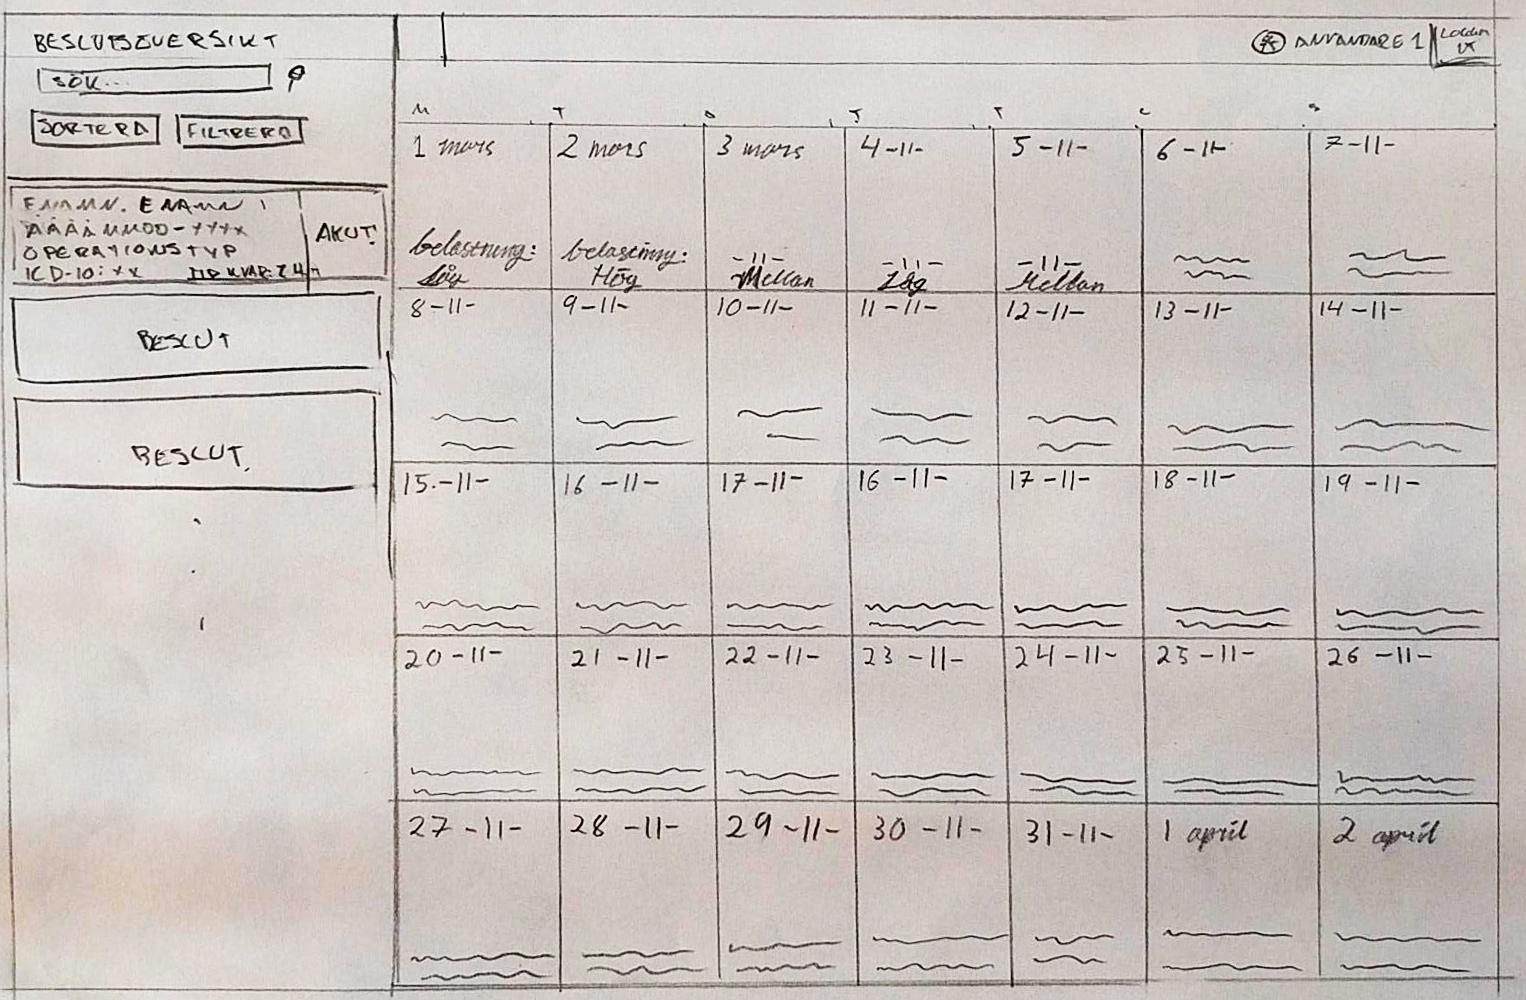
\includegraphics[width=\linewidth]{Figures/LoFi_no2.jpg}
  \caption{Sista LoFi-prototypen}
  \label{fig:LofiPic}
\end{figure}


Under projektets andra iteration utvecklades tre olika LoFi-prototyper. Dessa
LoFi-prototyper designades för att visa på olika designalternativ på
användargränssnittet. Ett exempel på detta är informationen som var med i listan
över beslutade operationer.

I en av prototyperna identifierades patienten som hörde ihop med beslutet med namn, den andra med personnummer. I den tredje LoFi-prototypen
fanns inget som identifierade patienten utan enbart information om vilken
typ av operation det var. På liknande sätt utvärderades olika sätt att
visualisera lediga tider i schemat samt olika sätt att anpassa sökparametrarna för en sökning efter lediga tider.

När prototyperna visades för kunden kunde alternativen sållas bort och en tydligare bild av behoven framträdde.
Till exempel fanns det endast personnummer och inte namn på patienterna, vilket var något som önskades.

Den första iterationen av LoFi-prototyper användes sedan för att ta fram en ny
LoFi-prototyp med enbart mindre designalternativ som visades för tre olika
operationsplanerare. (Figur \ref{fig:LofiPic} illustrerar en bild av den sista Lofi-prototypen.)

\subsection{Systemanatomi}
I första iterationen togs det fram en systemanatomi (se figur \ref{fig:Systemanatomi}) som användes under projektets gång som ett hjälpmedel för strukturera upp arbetet under utvecklingen. Den gav en översiktlig bild av vilken funktionalitet produkten skulle innehålla och hur de olika delarna samverkade med varandra. Utöver detta presenterades den i ett tidigt skede för kunden i syfte att säkerställa att projektgruppens syn på systemet stämde överens med kundens.

\begin{figure}[H]
    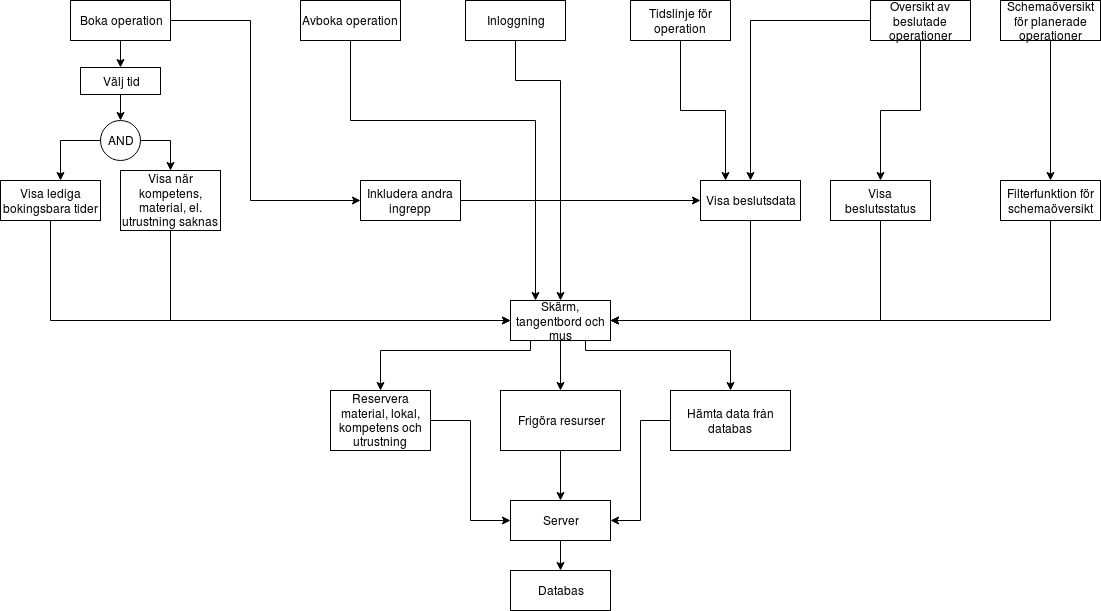
\includegraphics[width=\textwidth,height=.4\textheight]{Figures/Systemanatomi.png}\\
    \caption{Systemanatomi}
    \label{fig:Systemanatomi}
\end{figure}

\subsection{Värde för kund}
Den produkt som har skapats är ett lättöverskådligt schemaläggningssystem för operationer. Slutprodukten tillsammans med tankar och erfarenheter från design och utvecklings-faserna kommer att ha ett stort värde för kunden. Detta eftersom projektet kommer att användas som en form av förstudie till ett större projekt (se stycke \ref{sec:syfte}).

Det medför att Region Östergötland kommer att ha något att utgå ifrån då deras projekt startar, vilket hjälper av flera anledningar. Projektägaren som också är insatt i det större projektet kommer att kunna ta med sig många erfarenheter från det här projekt.

\section{Gemensamma erfarenheter}
Under projektet har medlemmarna fått stor erfarenhet av webbprogrammering då ingen hade någon större erfarenhet av detta sedan tidigare. Gruppen har fått sätta sig in i HTTP-protokoll, databaser och ett flertal programspråk och ramverk. Även versionshantering med git och gitlab har gruppen fått fördjupad kunskap inom. 

Vid utveckling av front-end lärde sig gruppen att använda ramverket Angular och att programmera i HTML, CSS och TypeScript. I back-end behövde medlemmarna istället sätta sig in i JavaScript, MySQL-databas och miljön Node.js med ett flertal tillhörande bibliotek.

Förutom tekniska erfarenheter har gruppen fått en större förståelse för hur sjukvården fungerar och att ett bra it-system kan göra stor verklig skillnad. Gruppen har även fått praktiskt erfarenhet av att utöva scrum. Det har varit seminarier där presentation och opponering ingick.  

Slutligen så har de fått kunskap att utveckla något i grupp, där förkunskaper saknades eller var begränsade och som införskaffas allteftersom.   

\section{Översikt över individuella bidrag}
I denna delen presenteras deltagarnas individuella bidrag översiktligt.

\todo{Lägg till era rubriker och en kort synopsis här}
\subsection{Adam}
En studie i hur teamledarens roll går att applicera tillsammans med scrum-metodik.
\subsection{Björn}
Hur kan versionshantering användas effektivt för ett mindre mjukvaruutvecklings projekt.
\subsection{Christoffer}
Betydelsen av att samla krav från en varierad grupp aktörer
\subsection{Henrik}
För/nackdelar med TypeScript jämfört med JavaScript
\subsection{Martin}
Angular som webbutvecklingsplattform
\subsection{Niclas}
Prototypuveckling i kandidatprojekt
\subsection{Tor}
Kvalitetsförsäkrande metoder i ett småskaligt mjukvaruprojekt

\chapter{Diskussion}
Detta kapitel tar upp diskussioner om resultatet av projektet och den metod som använts.
\section{Resultat}
Saker som kan tas upp:
\begin{itemize}
\item Fanns alternativa implementationssätt?
\item Vad återstår för att kunden skall få ut fullt värde av produkten?
\item Lyckades ni förbättra/fortsätta något från tidigare projekt
\item Viktigaste lärdomar inför framtiden.
\end{itemize}

\section{Metod}
Saker som kan tas upp:
\begin{itemize}
\item Vilka konsekvenser fick de valda metoderna för resultaten?
\item Fanns det alternativ?
\item Källkritik
\end{itemize}

\section{Arbetet i ett vidare sammanhang}
Saker som kan tas upp:
\begin{itemize}
\item Samhälleliga aspekter
\item Miljöaspekter
\item Etiska aspekter
\end{itemize}
\chapter{Slutsatser}
I detta avsnitt ska de frågeställningar som ställts i början av rapporten besvaras.

\textbf{Hur kan systemet som utvecklats implementeras så att värde skapas för kunden?}

Systemet som utvecklats kan bytas ut mot det nuvarande systemet för att få en tydligare grafisk vy över de operationer som är planerade. Det utvecklade systemet ger också ett enkelt sätt att boka in nya operationer på datum och tider där all kompetens, utrustning och material finns tillgängligt.

\textbf{Hur kan man separera front-end och back-end på ett bra sätt så att delarna inte är beroende av varandra?}
För att separera på back-end och front-end så att de kan utvecklas parallellt kan man först definiera ett tydligt API för all kommunikation som kommer att ske mellan dem. När API:et är färdigt kan detta implementeras på back-end i projektet. Efter detta, eller innan om API:et är väldefinierat, kan en modul skapas på front-end som definerar all funktionalitet som krävs för att använda detta API. Nu kan de två delarna fortsätta utvecklas separat så länge API:et inte ändras, och när detta händer är det endast komunikationsmodulen på front-end som behöver uppdateras.

\textbf{Vilka erfarenheter kan dokumenteras från projektet som kan vara intressanta för framtida projekt?}

Under projektets gång så har gruppen fått flera värdefulla erfarenheter. Den största erfarenheten är hur det är att arbeta i projekt med en större grupp människor och hur det är att arbeta med en agil utvecklingsmetod. Att arbeta mot en kund har också varit en bra erfarenhet då detta inneburit extra moment, som kundmöten och demonstrationer av programvaran, till skillnad från ett vanligt skolprojekt.

\textbf{Vilket stöd kan man få genom att skapa och följa upp en systemanatomi?}

Skapandet av en systemanatomi ger upphov till diskussion om vilka huvudfunktioner som ska finnas och hur systemet i helhet ska hänga ihop. Systemanatomin visar upp beroenden mellan olika delar av systemet och ger under systemutvecklingen en överblick av vilken funktionalitet som måste vara färdig innan annan kan testas. Anatomin hjälper till att ge en gemensam syn på systemet både inom projektgruppen och mellan gruppen och kund. Kunden fick genom systemanatomin möjlighet att i ett tidigt skede av projektet kontrollera om projektgruppen förstått uppgiften rätt.    


\part{Individuella bidrag}
\appendix
\chapter{Teamledarens roll kombinerat med scrum-metodik av Adam Andersson}

\section{A.1 Inledning}
Scrum modellen är ett välkänt arbetssätt som ofta används inom mjukvaruutveckling. I en grupp som använder sig utav Scrum-metoden så finns det ingen specifik ledare, om man bortser från scrum master som har ansvaret för att se till att Scrum-metodiken används, då alla är utvecklare och gruppen bestämmer tillsammans vad som ska göras och hur problem ska lösas.
I detta projektet har även alla gruppmedlemar en projektroll varav en person innehar rollen som teamledare. Denna studie ska utreda hur rollen som teamledare fungerar i kombination med scrum-metodik.

\subsection{A.1.1 Syfte}
Rollen som teamledare innebär att du ska coacha projektgruppen och se till att de mål som finns för projektet uppfylls. Enligt scrum-metodik så är det gruppen som tillsammans ska bestämma över de beslut som tas och hur problem ska lösas. Syftet med denna studie är att utreda om det går att kombinera rollen som teamledare med scrum-metodik.

\subsection{A.1.2 Frågeställning}
Utefter det syfte som denna studie har ska följande frågor försöka besvaras:

\begin{enumerate}
	\item Hur ser teamledarrollen ut?
	\item Hur fungerar scrum-metodik?
	\item Går det att kombinera teamledarrollen i en scrum-metodik och fortfarande bibehålla syftet med de båda? 
\end{enumerate}

\section{A.2 Bakgrund}
I början av projektet skulle gruppen tilldela samtliga medlemmar en roll, däri fanns rollen teamledare som författaren av denna studie tog på sig. När projektet hade fortgått i några veckor så togs det upp vilken metodik gruppen skulle använda för projektet. Kunden föreslog att vi kunde använda oss av scrum, så teamledaren läste på om denna metodik och höll en redovisning för gruppen. Efter redovisningen diskuterades om detta verkade vara en bra metod. Då scrum är en välkänd agil utvecklingsmetod med enkla och strukturerade riktlinjer så tog gruppen beslutet att använda sig av denna. När gruppen började använda sig av metodiken så började jag fundera över hur detta skulle påverka rollen som teamledare då teamledaren är en typ av ledarroll men enligt scrum så är det gruppen som tar beslut om vad som ska göras och hur problem ska lösas.

\section{A.3 Teori}
Detta avsnitt går igenom den teori som finns till grund för denna studie.

\subsection{A.3.1 Scrum} \label{adam_scrum}
Scrum är en arbetsmetodik som främst används för mjukvaruutveckling. Metodiken appliceras på mindre team (3-9 personer) och går ut på att teamet arbetar i tidsbestämda sprintar där det existerar ett antal uppgifter som ska genomföras under respektive sprint.
I scrum så existerar ett fåtal specifika roller som används för att beskriva de inblandade i projektet. De roller som existerar är:

\begin{itemize}
	\item \textbf{Produktägare}
	
	Produktägaren är den person som representerar beställaren, vanligtvis aktieägarna i större bolag, och förmedlar till utvecklingsteamet vilka krav som finns och vilka av dessa som har högst prioritet. En viktig egenskap för en produktägare är empati, du arbetar med aktieägare som ofta har olika bakgrund och värderingar. Produktägaren måste också vara bra på att samarbeta med utvecklarna så att arbetet med produkten går bra och att krav uppfylls.
	
	\item \textbf{Scrummästare}
	
	Scrummästaren skiljer sig från den klassiska teamledaren eller projektledaren. Dess roll är att se till att det inte existerar några hinder för utvecklingsteamet så att de kan uppnå projektmål och leverera en produkt. En annan viktig uppgift för scrummästaren är att se till att de processer som man valt att applicera i scrum-metoden utförs och efterföljs. Samarbete med produktägaren finns också för att underhålla backloggen så att utvecklingsteamet förstår vad som ska göras och så att arbetet med produkten kan fortgå.
	
	\item \textbf{Utvecklingsteam}
	
	Utvecklingsteamet är själva projektgruppen och den ansvarar för att göra framsteg i arbetet och utföra de uppgifter som existerar i respektive sprint. Trots att det kan finnas olika typer av roller så kallas alla i teamet för utvecklare. För att inte skapa förvirring så kallas utvecklingsteamet för leveransteam och personerna för teammedlemmar.	
\end{itemize}

Utöver de roller som existerar i scrum så använder man sig också av fyra olika mötestyper som inträffar med olika frekvens. Det viktiga med dessa möten är att de är tidsbestämda och den maximala tid som ska läggas på dessa beror i flera fall på hur lång en sprint i projektet är, detta för att man inte ska lägga alltför lång tid på möten. De mötestyper som existerar är:

\begin{itemize}
	\item \textbf{Sprintplanering (maximalt 4 timmar för en tvåveckors-sprint)}
	
	Sprintplaneringen är uppdelad i två delar, den första delen går ut på att produktägaren, scrummästaren och utvecklingsteamet väljer de uppgifter från backloggen som man tror kommer hinnas med under den kommande sprinten. När detta är gjort så kommer planeringens andra del, utvecklingsteamet diskuterar och kommer mer specifikt fram till vilka arbetsuppgifter som behöver göras för att uppgifterna från backloggen ska kunna utföras och uppfyllas. Denna andra iteration över uppgifterna kan leda till att man delar upp vissa uppgifter eller att vissa uppgifter läggs tillbaka i backloggen då man inte tror att dessa kommer hinnas med under kommande sprint.
	
	\item \textbf{Daglig scrum (maximalt 15 minuter)}
	
	Varje dag hålls ett dagligt scrum-möte för att uppdatera utvecklingsteamet om vilka framsteg och hinder som finns i sprinten så att teamet kan öka sina chanser att nå målen med nuvarande sprint. Dessa möten är tidsbestämda till 15 minuter och de kan utföras stående i en ring, så att man inte fokuserar på annat och så att man håller sig inom de 15 minuterna. Man kan utgå ifrån tre frågor under en daglig scrum:
	
	\begin{itemize}
		\item Vad har jag gjort sedan igår?
		\item Vad ska jag åstadkomma till imorgon?
		\item Vad hindrar mig?
	\end{itemize}
	
	Om det skulle komma fram att det finns några hinder i gruppen så ska scrummästaren notera detta och man bör sätta en person på att lösa problemet så att sprinten kan fortgå utan hinder.
	
	\item \textbf{Sprintgenomgång (maximalt 2 timmar för en tvåveckors-sprint)}
	
	När en sprint är avslutad hålls en sprintgenomgång, där man tittar på vilka arbetsuppgifter utvecklingsteamet har, och inte har, hunnit med att slutföra. Man håller också en demo för beställaren där man visar vilka framsteg som har gjorts under sprinten. Efter genomgång av utförda och icke utförda arbetsuppgifter samt demo så diskuterar utvecklingsteamet och beställaren vad teamet ska arbeta med härnäst.
	 
Det som är viktigt att tänka på under en sprintgenomgång är att man inte ska visa upp arbetsuppgifter som inte är färdiga, t.ex. ska man inte visa upp funktionalitet i ett program om funktionaliteten inte är helt färdig.

\item \textbf{Sprintåterblick (maximalt 90 minuter för en tvåveckors-sprint)}

När en sprintgenomgång har utförts är det dags för en sprintåterblick. Sprintåterblick innebär att man utvärderar den sprint som har varit genom att utgå från två frågor:

\begin{itemize}
	\item Vad gick bra under sprinten?
	\item Vad kan förbättras till nästa sprint?
\end{itemize}

Från dessa två frågor så identifierar man förbättringar som kan göras. Man väljer ut några av dessa punkter och arbetar med dem i nästa sprint.

\end{itemize}
https://en.wikipedia.org/wiki/Scrum_(software_development)

\subsection{A.3.2 Teamledarrollen}
Teamledaren är den person som ska coacha teamet mot de mål som är uppsatta. Du är lyhörd och ser till att alla känner sig delaktiga i processen. Teamledaren är inte en projektledare och kan därför ta ett steg tillbaka i ledarrollen för att få medlemmar i gruppen att ta plats och utvecklas.\cite{teamledare} Trots att teamledaren kan ta ett steg tillbaka så är personen ändå närvarande i gruppen och ser till att ha täta avstämningar för att ha koll på vad som händer och för att skapa samhöriget inom gruppen.\cite{teamguide}

\section{A.4 Metod}
För att genomföra denna studie har tre olika metoder använts. Informationssökning genom att leta efter vetenskapliga artiklar som analyserar scrum-metoden, egna erfarenheter genom att analysera hur arbetet i projektgruppen har fortgått och intervjuer av medlemmar i andra projektgrupper som också har använt sig av scrum-metoden.

\subsection{A.4.1 Informationssökning}
Det finns en artikel som handlar om att förstå och arbeta med delat ledarskap i agil utveckling. \cite{sharedleader}

I den studien har man följt ett företag som nyligen har börjat använda sig av scrum-metoden för att se hur det fungerar i praktiken att dela upp ledarskap bland alla inblandade parter. Det man kunde observera var att medlemmarna i det projekt som observerades inte kunde lägga så mycket tid på projektet som man planerat, detta för att de var involverade i andra projekt som var beroende av dem. Ett annat problem man kunde se var att det saknades kompetens eller vilja att ta ledarrollen, en roll som ska roteras i scrum till den som har mest kompetens. \cite{sharedleader}

\subsection{A.4.2 Egna erfarenheter}
Under projektet som genomförts så hade jag rollen som både teamledare och scrummästare. Det gav både erfarenhet i att leda en grupp i ett projekt och att hålla koll på de olika processer som används inom scrum.

\subsection{A.4.3 Intervjuer}
Intervjuer har utförts på ett antal studenter som läser kursen TDDD96. För att få in ett bredare spektrum av erfarenheter om hur det är att arbeta med scrum och en teamledare har intervjuerna utförts på personer från olika projektgrupper.

Intervjuerna gick ut på det sättet att jag presenterade den studie jag arbetade och sedan ställde jag ett antal frågor. Till att börja med ställde jag frågor om vilken roll de hade i projektet, sedan följde frågor om varför de valt scrum, om personen var scrum-master och hur det fungerat med att upprätthålla dessa processer. Slutligen så ställde jag frågor om teamledarrollen, hur den tillämpats i projektet och hur det har gått att kombinera den med scrum-metodik. De frågor som ställdes till till de som intervjuades var:

\begin{enumerate}

\item Vilken roll har du i projektet?

\item Hur kommer det sig att ni valde att arbeta med scrum?

\item Vilka delar av scrum har ni tillämpat?

\item Vilken roll i er projektgrupp är scrummästare?

\item Varför valde ni just den rollen som scrummästare?

\item Hur har det gått med att upprätthålla scrum-processerna?

\item Vilka uppgifter har teamledaren i er projektgrupp?

\item Hur har kombinationen av teamledare och scrum-metodik fungerat?

\item Har rollen som teamledare och scrum-metodik gynnats av varandra?

\item Finns det något man kan ändra på i teamledarrollen eller i scrum-metodik för att arbetet skulle kunna förbättras?

\item Har du något övrigt att tillägga?

\end{enumerate}

\section{A.5 Resultat}

\section{A.6 Diskussion}

\section{A.7 Slutsatser}


\chapter{Prototyputveckling i ett kandidatprojekt av Niclas Byrsten}\label{appendix:prototyp}

\section{Inledning}
Innan ett mjukvaruprojekt kommer in i själva utvecklingsfasen så är det viktigt att både kunden och projektmedlemmarna har samma bild av hur slutproduktens grafiska gränssnitt ska vara utfoemat. Det finns många olika metoder och verktyg som kan vara till hjälp där en av dessa är prototypning.  

\section{Syfte}
Syftet med den här rapporten är att beskriva hur arbetsgången med prototyper utfördes av projektgruppen under och vilka slutsatser som kan dras utifrån det.  

\section{Frågeställningar}
De frågeställningar som rapporten ska besvara är:
\begin{enumerate}
    \item Vilka fördelar och nackdelar finns det med prototypning?
    \item Hur effektivt är prototypning vid ett mindre projekt?
\end{enumerate}

\section{Bakgrund}
Ett inte allt för ovanligt problem som finns då ett gränssnitt ska tas fram är att det kan uppstå problem i kommunikationen mellan projektgruppen som ska utveckla systemet och övriga aktörer med intresse i projektet såsom beställare och slutanvändare. En prototyp används vanligen för att dela ideer om designen men även för att överbrygga detta gap som kan finnas mellan tidigare nämnda grupper \cite{caseStudy}. Den kan ses som ett hjälpmedel eller verktyg för att säkerhetsställa att det system som ska tas fram stämmer överens med de krav och förväntningar som kan finns på systemet. På ett tydligt sätt så går det att hur projektgruppen föreställer sig att att slutprodukten ska se ut och det går i ett tidigt stadie ge både åsikter och synpunkter. På samma gång så kan det även hjälpa projektgruppen att få sig en tydlig bild av hur den grafiska designen kommer att bli utformad. 

\section{Avgränsningar}
Denna rapport kommer endast belysa erfarenheter och slutsatser som kan dras med utgångspunkt från det här projektet.

\section{Teori}
Nedan så presenteras den teori som denna rapport bygger på.

\section{Prototyp}
En prototyp är en arbetsmodell vars syfte är utveckla och testa design ideer. Två typer av prototyper som är vanligt förekommande är low-fidelity och high-fidelity. I den efterföljande texten så  kommer dessa att benämnas som lo-fi prototyp respektive hi-fi prototyp. Uttrycket fidelity beskriver hur prototypen skiljer sig ifrån och hur väl den representerar den slutgiltiga produkten \cite{prototypeChoise}.Den kan sägas vara en simulering av slutprodukten.     

\subsection{lo-fi prototyp}
En lo-fi prototyp skiljer sig ifrån den slutgiltiga produkten på punkter som detaljrikedom, interaktion och utseendemässigt. De kan vara gjorda av papper och de största fördelarna är att de är snabba att skapa, enkla att vidareutveckla  och de kan flytta fokus till själva interaktionsdesignen istället för detaljer och visuell styling \cite{prototypeChoise}.

\subsection{hi-fi prototyp}
En hi-fi prototyp är mer lik slut produkten.  I jämförelse med en lo-fi prototyp så erbjuder en hi-fi prototyp mer realistiska interaktioner, fler detaljer, är mera lik slutprodukten och förmedlar bättre vilka designmöjligheter som kan erbjudas. De är dock mer kostsamma och tar längre tid att konstruera \cite{prototypeChoise}.

\section{Val av Prototyp} 
Under projektet har gruppen tagit fram ett flertal pappersprototyper där vissa  har demonstrerats för kunden. I ett tidigt skede så hade kunden framfört önskemål om att projektgruppen skulle använda sig av pappersprototyper. Gruppens medlemmar hade tidigare läst en kurs i interaktiva system där de bland annat gjorde en pappersprototyp som sedan vidareutvecklades till en hi-fi prototyp med hjälp av digitala mjukvaruverktyg. Men ingen hade erfarenhet av att gå ifrån pappersprototyp till färdig produkt. Att använda sig av pappersprototyper tidigt innan någon kod har skrivits är både billigare och mer tidsbesparande än att göra ändringar senare \cite{paper}. Under detta projekt så fördes även diskussion om gruppen skulle göra en hi-fi prototyp med något digital verktyg innan själva utvecklandet av produkten tog sin början. Men det var inget som gjordes då det upplevdes räcka med pappersprototyper och att det inte var värt den tidsinvestering som krävts.      

\section{Förberedelse}
Efter ett av de första mötena med kunden, där kravspecifikationen togs fram, så hade gruppen ett möte om hur den grafiska designen för produkten  skulle se ut. Då ingen i projektgruppen hade någon riktigt klar bild av hur den skulle vara utformad så kom gruppen överens om att varje person skulle skissa på en egen prototyp av hur det grafiska designen skulle kunna se ut. Tanken med detta var att kunna få fram så många olika förslag som möjligt då. Varje förslag visades för upp för resten av gruppen som kom med frågor och gav sina tankar om den. Efter alla designförslag hade presenterats så hölls en diskussion om var och en av föslagen, där det tillslut valdes ut två stycken förslag som förbättrades och skulle visa på olika alternativ på hur gruppen tänkte sig att den slutgiltiga versionen skulle kunna se ut. Ett nytt möte bokades in med kunden för att få återkoppling. Utöver dessa två så togs det även med en tredje prototyp som hade gjorts efter diskussion tillfället som inte var helt fullständig men som kunde visa olika alternativ på enskilda komponenter i gränssnittet.

\section{Första mötet}
På mötet så närvarade fem stycken personer från kundens sida och fyra stycken från projektgruppens sida. Inledningsvis så introducerade gruppen prototyperna och berättade hur de föreställde sig att den skulle se ut.  De två första prototyperna testades genom att en av dessa fem fick agera testperson med uppgift att boka in en operation samtidigt som testpersonen berättade vad den såg och hur. Under mötet så fördes även en fortlöpande diskussion om vad som var bra och vad som borde förbättras. När tillfälle fanns så gav även de övriga personerna som var närvarande sina åsikter och synpunkter. Många av de frågetecken som fanns innan reddes ut och det blev mer tydligt vad kunden hade för förväntningar. 

\section{Andra mötet}
Efter det  så samlades gruppen för att diskutera vad som hade framkommit under föregående möte och hur nästa prototyp skulle byggas. Några av dessa punkter  presenteras nedan:
\begin{enumerate}
	\item Det ska finnas en bekräftelseruta med en total sammanfattning över alla detaljer i bokningen innan man 	 			  	  bekräftar bokningen.
 	\item Det ska stå namn på patienten i listan över beslut, eller åtminstone initialer.
 	\item Det är ett intressant koncept att visa detaljer om en bokning i form av en tidslinje
 	\item Under översikten över lediga tider kan någon form av spårsystem vara intressant att utveckla.
\end{enumerate}
Två personer blev ansvariga för konstruktionen som visades upp för de andra innan den ansågs redo. Denna gång skulle den presenteras för tre personer som i skrivande stund arbetar som schemaläggare på tre olika avdelningar. Det sågs som positivt att testa på fler slutanvändare då de kan ha olika syn på vad som borde finnas med och hur det ska se ut. Från projektgruppen närvarade tre personer. Inledningsvis så presenterades prototypen och hur gruppens tankar om hur den skulle fungera. Efter det så framförde schemaläggarna sina tankar och åsikter. Precis som under första mötet hölls en kontinuerlig diskussion.
Återigen så hölls ett nytt gruppmöte om det som framkommit och hur prototypen skulle förbättras. Gruppen ansåg att det fanns en tillräckligt bra grund för att börja implementera designen av det grafiska gränssnittet.      
  
\section{Metod}
Den här rapporten bygger på författarens egna upplevlser och diskutioner som har skett inom gruppen. Vidare så gjordes en intervju med gruppens medlemmar för att få en samlad bild av gruppens erfarenheter och synpunkter. Nedan listas de frågor som ställdes:
\begin{enumerate}
	\item Vad tycker du har gått bra med att använda sig av prototyper?
 	\item Är det något du tycker har fungerat mindra bra?
 	\item Vad det värt den tid det tog?
 	\item Hur har du haft användning av prototypen i projektet?
 	\item Har det hjälpt dig att få en bättre uppfattning hur det grafiska ska se ut?
 	\item Skulle du använda dig av prototyper i ett liknande projekt i framtiden? 
\end{enumerate}
 
\section{Resultat}
Utifrån de intervjuerna så erhölls några intressanta svar. Bland annat så skulle alla medlemmar använda sig av prototyper i ett liknande projekt i framtiden och det var värt den tid det tog. Alla utom en tycker att de har haft nytta av den i projektet. De fördelar som nämndes var exempelvis att prototypen var snabb och enkel att göra, många olika ideer fångades upp i gruppen. Bland det negativa finns saker som att den inte var så interaktiv och att det kan vara svårt att visa på vad som är tryckbart. Utöver det så upplevde gruppmedlemmarna att prototypen varit till hjälp vid implementatione av grafisk komponenter. Svaren på alla frågor återfinns i appendix J.  
  
\section{Diskussion}
Under projekt testades fyra pappersprototyper mot tilltänkta slutanvändare. Under dessa tillfällen så användes prototypen för att tydliggöra gruppens bild av den grafiska designen. Den återkoppling som erhölls blev klarare och möjliggjorde en bättre kommunikation. I ett tidigt skede kunde gruppen åtgärda designfel som annars kan ha missats eller upptäckts först när implementationen hade börjat. De oklarheter som fanns i början blev tyligare. Under projektes gång så gick det alltid att blicka tillbaka på prototypen.
Överlag så verkar alla gruppmedlemmar vara nöjda prototypningen. Vissa saker hade kunnat gjorts annorlunda.  


\section{Slutsats}


\chapter{Versionshantering för ett mindre mjukvaruutvecklingsprojekt - Björn Hvass}


% Tankar
%
%
%
%
%
%
%
%
%
%
%

\vspace{3em}
\section{Inledning}
Inför ett mjukvaruprojekt är det kritiskt att välja rätt versionshanteringsprogram. Programmet måste på ett bra sätt skala till projektets storlek, den funktionalitet som planeras att användas och inlärningskurvan för programmet måste vara lämpligt. Den här rapporten tillhandahåller information erhållen genom analys av intervjuer angående valet och effektiviteten av olika versionshanteringsprogram för mindre mjukvaruutvecklingsprojekt.

\section{Syfte}
Syftet med den här rapporten är att undersöka hur versionshantering kan användas i ett mindre mjukvaruutvecklingsprojekt. Rapporten analyserar olika arbetsmetodiker i syftet att utreda om en metodik kan användas tillsammans med en mindre projektgrupps arbetssätt på ett effektivt sätt.

\section{Frågeställning}
\begin{enumerate}
    \item Vilka olika verktyg och arbetsmetodiker används för versionshantering i mindre mjukvaruutvecklingsprojekt?
    \item Går det att säkerställa att en projektgrupp arbetar effektivt med versionshantering?
\end{enumerate}

\section{Avgränsningar}
Rapporten kommer endast utföra sin undersökning, intervjuer, på personer som studerar eller studerat vid Linköpings universitet på en datainriktad utbildning. Detta eftersom det blir enklare att finna lämpliga personer att intervjua då det finns mer direkta kanaler att använda för att finna personer att intervjua. Vidare så finns det en viss garanti för att personen har arbetat i mindre mjukvaruprojekt.

\clearpage
\section{Bakgrund}
Inför kandidatprojektet för linjen, civilingenjör i datateknik, på Linköpings universitet beslutade sig min projektgrupp sig för att använda versionshanteringsprogrammet Git.
Webbtjänsten som valdes för att hantera projektgruppen data var GitLab. Gruppen valde Gitlab eftersom institutionen för datavetenskap vid Linköpings universitet tillhandahåller alla studenter med sin egen GitLab-server. Alla studenter har automatisk tillgång till serven utan avgifter.

Att använda Git möjliggör för det första att gruppen på en enkelt och familjärt sätt kan monitorera ändringar i de filer som versionshanteras, i vårt fall både programkoden och dokumentationen för projektet. Dokumentationen versionshanteras då LaTeX valts som typsättningssystem och Git var ett smidigt sätt att versionshantera LaTeX-filer. För det andra så har Git också stöd för utveckling av olika versioner av samma kod parallellt. Det gör genom något som kallas grenar. Det gör att gruppens medlemmar kan arbeta på olika uppgifter samtidigt utan att vara till besvär för varandra.


\section{Teori}
Det här avsnittet redogör för den teori som är relevant för rapporten.
\subsection{Versionshantering}
Versionshantering är i grunden ett sätt att hantera förändringar och säkerhetskopiera data, vanligtvis handlar det om programkod men kan användas för alla typer av filer. Ingen skulle idag lämna data som är viktig utan att säkerhetskopiera den, att det sedan finns versioner av datan sparade är en stor fördel då det är svårt att mista data. Vissa typer av data, till exempel programkod, har en tendens att ändras mycket under sin livstid. Det blir då väldigt viktigt att kunna hantera alla ändringar och till exempel gå tillbaka till en tidigare version om det skulle behövas. Då versionshantering medför flera fördelar så har det idag blivit en naturlig del av en mjukvaruutvecklares vardag.\cite{VersionControlGit}

Inom versionshantering är det varligt att projekt delas upp i olika grenar, där varje gren har ett specifikt syfte. Projektet har vanligtvis en huvudgren som ofta kallas master på engelska och mästare på svenska. Huvudgrenen ska endast innehålla färdig implementerad och testad funktionalitet.
En gren är som en sorts kopia av en annan av projektets grenar, vanligtvis av huvudgrenen. När en gren har skapats så kan ändringar utföras oberoende av ändringar på andra grenar. Det betyder att flera personer kan arbeta på olika saker så som ny funktionalitet eller buggfixar parallellt. När en gren har uppnått sitt syfte så kan den inkorporeras med projektets huvudgren och bli en del av produkten.

De tre populäraste kostnadsfria versionshanteringsprogrammen är Git, Subversion och Mercurial. Git är det mest populära programmet och Subversion och Mercurial delar andra plats.\cite{version_comp}
\subsubsection{Git}
Git är ett distribuerat versionshanteringsprogram som har snabbhet, dataintegritet och stort stöd för distribuerade olinjära arbetsflöden som huvudfokus. Att det är distribuerat betyder att alla användare har en lokal kopia av hela projektet som sedan kan synkroniseras med gruppens gemensamma kopia av projekt som ligger på en server. Två av de största webbtjänsterna som tillhandahåller Git-servrar är GitHub och GitLab.\cite{VersionControlGit}\cite{web_Git}

\subsubsection{Mercurial}
Mercurial är ett distribuerat versionshanteringsprogram vars mål inkluderar att det ska vara lätt att använda sig av och lära sig. Det ska också vara skalbart i förhållande till projektets storlek och behov. Vidare var det designat för stödja en mångfald av operativsystem då mycket av programkoden är skriven i Python och bara små delar i C.
\cite{VersionControlMercurial}\cite{VersionControlMercurial}


\subsubsection{Apache Subversion}
Apache Subversion är ett centraliserat versionshanteringsprogram, programmet benämns ofta som SVN efter sitt terminalnamn svn. SVN är från börjar utvecklat med syftet att ersätta Concurrent Versioning System som släpptes 1990. Ett centraliserat system använder sig av en server där all data sparas.\cite{wiki_cvs}\cite{VersionControlSvn}\cite{web_Svn}


\section{Metod}
För att undersöka vilka olika verktyg och arbetsmetodiker som är attraktiva i mindre mjukvaruutvecklingsprojekt har intervjuer utförts. I undersökningen har studenter som går eller slutfört ett civilingenjörs kandidatarbete eller liknande intervjuas. Även ingenjörer på mindre företag som arbetar i mindre projekt har att sköts.

Intervjuerna fokuserar på att samla in information angående vilket versionshanteringsprogram som den intervjuade personens projektgrupp använde och varför. Vidare var det också av intresse att samla in information angående vilken arbetsmetodik som guppen använde när det gäller versionshantering. Det är också intressant varför just den metodiken valdes och om den passade gruppens arbetssätt.

%Finns mycket teori angående workflow, förhoppningsvis även en del studier.
\subsection{ Intervjufrågor } \vspace{1em}
\begin{enumerate}

  \item Kan du kort beskriva ett mindre mjukvaruutvecklingsprojekt som du har medverkat i? Vad var syftet med projektet?

  \item Vilket versionshanteringsprogram användes under projektet?

  \item Hade ni möjligheten att välja?

  \item Följdfråga om föregående fråga sant: Hur kommer det sig att ni valde just det ni gjorde?
  \item Följdfråga om föregående fråga falskt: Hur påverkade det projekt?

  \item I projekt hade ni en arbetsmetodik för versionshantering, om så var fallet hur fungerade den?

  \item Använde sig gruppen av metodiken så som det var tänkt i teorin?

  \item Passade metodiken storleken på gruppen?

  \item Använde gruppen något speciellt ramverk eller arbetssätt för att hantera arbetsprocessen och planera arbetet, t.ex. Veckomöten, Scrum?

  \item Följdfråga: Vävde ni samman arbetssättet med versionshanteringen och arbetsmetodiken på något sätt?

  \item Skulle du säga att arbetsmetodiken för versionshanteringen som ni använde var effektiv? Varför?

  \item Hur tycker du att programmet i sig fungerade i projektet?

  \item Var det svårt att lära sig versionshanteringsprogrammet? Fanns det programvara som gjorde versionshanteringen blev lättare att hantera?

\end{enumerate}

\section{Resultat}
Under undersökningen intervjuades sex olika studenter som hade tidigare erfarenhet av att arbeta i mindre mjukvaruutvecklingsprojekt. Där projektgruppen för respektive projekt använde sig av versionshantering. Bilaga \ref{appendix:bjorn} innehåller intervjuerna, på grund av att svaren i en av intervjuerna inte kunde publiceras så har den intervjun exkluderats från bilagan.

Utifrån intervjuerna så framgick det att den klara majoriteten använde sig utav versionshanteringsprogrammet Git. Vilken webbtjänst som de olika projektgrupperna använde sig av för att lagra och hantera den data som versionshanterats skiljde sig dock åt. En av de som blev intervjuade använde sig av SVN, Apache Subversion, för versionshantering.\cite{VersionControlSvn}

Det framgick också att de som arbetade i studentprojekt och hade möjligheten att välja versionshanteringsprogram själva, gärna valde Git på grund av den breda funktionalitet och popularitet programmet har bland studenter på Linköpings universitet. Det enda andra programmet som användes var SVN, detta användes i samband med ett jobb där det var standard på företaget att använda SVN.

Alla använde sig av någon form av arbetsmetodik för versionshanteringen och vävde samman versionshanteringen med andra naturliga aspekter inom mjukvaruutveckling som testning och kodinspektioner. Personen som använde SVN hade den lättaste metodiken i sitt arbete, där användes versionshantering mer som ett sätt att säkerhetskopiera och testa programkod. För att lösa problem som uppstod med SVN tog personen till egna, mer praktiska metoder, istället för att använda SVN:s funktioner som det var tänkt.

 När det gäller Git planerade alla att använda sig utav någon form av ``Feature Branch Workflow'', vilket kan beskrivas som ett arbetssätt med funktionalitetsförgrening för Git. Det visade sig att alla som använde sig av Git hade valt eller utformat en arbetsmetodik som passade gruppen kompetens, storlek samt behov. Av den anledningen så användes ofta arbetsmetodiken i praktiken som det var tänkt i teorin.

 Det framgick också att när det fanns en formulerad arbetsmetodik för versionshantering så användes den på ett effektivt sätt då gruppens medlemmar förstod syftet med metodiken och hur versionshanteringsprogrammet fungerade.

Det framgick också i fem av sex intervjuer att gruppen behövde ta sig över en viss upplärningskurva för att komma igång med versionshanteringen. Detta då inte alla i de berörda grupperna hade kommit i kontakt med de mer avancerade aspekterna av versionshantering tidigare.

\section{Diskussion}

Resultatet visade på att en klar majoritet använder sig av Git för versionshantering. Alla som hade möjligheten av välja vilket verktyg de skulle använda för versionshantering valde Git. Utav de som inte fick välja utan blivit tilldelade Git så var det fortfarande Git det troligaste valet om de hade fått chansen att välja. Anledningen till det var att majoriteten av gruppen hade tidigare erfarenheter av Git. Det här kan tyda på att Git är ett väldigt populärt på Linköpings universitet där alla de intervjuade personerna studerar.

Då alla intervjuer hade färdigställts kunde ett mönster observeras bland svaren. Grupper vars medlemmar hade tidigare erfarenhet av versionshantering hade en tendens att välja en mer utförlig och avancerad arbetsmetodik. Denna arbetsmetodik arbetades också in i gruppens arbetssätt på ett mer framträdande sätt. Det visade sig också att dessa grupper ofta höll sig till metodiken så som det var tänkt när de arbetade.

Nästan alla som intervjuades uttryckte att det fanns medlemmar i gruppen som inte hade någon större erfarenhet av versionshantering innan projektet. Detta var dock inte ett problem då det fanns medlemmar som hade erfarenhet och kunde lära ut samt förklara hur versionshanteringen fungerade.

\section{Slutsatser}

Det visar sig att de flesta använder sig av Git som versionshanteringsprogram när det gäller mindre mjukvaruprojekt. Någon form av arbetsmetodik som använder sig av grenar används för att säkerställa att arbetet flyter på bra. Det visar sig också att då en grupp förstår syftet med arbetsmetodiken och hur versionshanteringsprogrammet fungerar så kommer versionshanteringen användas på ett effektivt sätt. Rapporten visar också på hur arbetsmetodiken för versionshantering kan vävas samman med en projektgrupps arbetssätt för att bli en naturlig del av arbetsprocessen.

\chapter{Jämförelse mellan TypeScript och JavaScript av Henrik Lindström}

\section{Inledning}
Vid utveckling av webbapplikationer är språkvalen något begränsade. I grunden är det dynamiskt typade JavaScript ofta det enda alternativet eftersom det är det enda scriptspråket med ett brett stöd av webbläsare. Vill man ha statisk typning så finns det dock alternativ som uppnår samma webbläsarstöd genom att kompileras till JavaScript. Ett av dessa är TypeScript som är en typad utökning av JavaScript. Under projektet användes delvis TypeScript och delvis JavaScript vid utveckling av webbklienten respektive webbservern.

I denna rapport undersöks hur de två olika språken och dess olika typsystem påverkade utvecklingsarbetet i projektet \textit{Schemaläggningsstöd för kirurgi} där en webbapplikation utvecklades.
\section{Syfte}
Denna rapport undersöker positiva och negativa effekter med användning av TypeScript jämfört med JavaScript. Mer specifikt är det de två språkens olika typsystem som ligger i fokus. Syftet med detta är att komma fram till vilka effekter statisk typning jämfört med dynamisk har på feldetektering, kodförståelse och utvecklingsfart.

\section{Frågeställningar}
För att uppfylla syftet kommer följande frågeställningar att besvaras i rapporten:
\begin{enumerate}
\item Bidrar den statiska typningen i TypeScript till att fel hittas tidigare under utveckling?
\item Bidrar den statiska typningen i TypeScript till kod som är lättare att läsa och förstå?
\item Hur påverkas produktivitet vid utveckling av statisk typning jämfört med dynamisk?
\end{enumerate}
\section{Bakgrund}
I projektet utvecklades en webbapplikation bestående av två delar, en webbklient och en webbserver. Eftersom det bestämdes att klienten skulle skrivas med hjälp av plattformen Angular medförde det också att språket TypeScript valdes. Detta eftersom Angular själv är skrivet i TypeScript. På serversidan bestämdes det istället att utvecklingen skulle ske med vanlig JavaScript. Både TypeScript och JavaScript användes alltså i projektet och en stor del av gruppen använde och fick i alla fall någon erfarenheter om båda. Alla medlemmar hade också svaga eller inga kunskaper om de båda språken innan projektet. Detta innebar att projektet lämpade sig rätt så bra för denna undersökning.

Jämförelse mellan strikt och dynamiskt typade språk är relevant eftersom det finns många språk på båda sidor som flitigt används inom mjukvaruutveckling. Detta tyder på att båda typsystemen är mycket relevanta och det är därför intressant att jämföra dem, i det här fallet inom webbutveckling.
\section{Teori}
I denna del beskrivs teori gällande de de två språken som jämförs i rapporten och deras olika typsystem.
\subsection{JavaScript}
JavaScript är ett dynamiskt och objektorienterat skriptspråk som främst används för att programmera interaktiva webbsidor och webbapplikationer. Språket kan även kan köras utanför webbläsare genom t.ex. miljön Node.js där det ofta används som skriptspråk för webbservrar. \cite{henrik_js1}

Språkets syntax delar många likheter med kända språk som Java och C++ men det finns också stora skillnader. En av dessa är att JavaScript är ett dynamiskt typat språk. Detta innebär att variabler i språket inte har någon speciell typ, istället är det värden som håller i typinformationen. Det medför att variabler inte har någon förutbestämd typ, utan kan byta mellan värden med olika typer. \cite{henrik_js2}

En annan stor skillnad är hur objekt hanteras i JavaScript. Det finns inga klasser utan endast objekt. Medlemsvariabler och funktioner för objektet skapas istället under körning, antingen vid skapandet av objektet eller vid senare tillfälle. \cite{henrik_js3}
JavaScript är även ett interpreterat språk \cite{henrik_js1} vilket innebär att det inte kompileras utan körs direkt som det är skrivet. Detta medför bland annat att ett program kan köras problemfritt trots att det innehåller fel i koden, så länge körningen inte kommer till den felaktiga delen.
\subsection{TypeScript}
TypeScript är ett skriptspråk utvecklat Microsoft som är en strikt syntatisk övermängd till JavaScript. \cite{henrik_ts1} Vad detta betyder är att allt som är giltig JavaScript-kod är även giltig i TypeScript, men att extra funktionalitet också finns tillgänglig. De största utökningar som gjorts är frivillig statisk typning och klasser.

För att ha ett lika brett stöd som JavaScript är TypeScript ett kompilerat språk som omvandlas till vanlig JavaScript. Att det är ett kompilerat språk tillsammans med statisk typning och klasser tillåter TypeScript att hitta typfel och andra mindre fel som felstavningar direkt vid kompilering.
\subsection{Dynamisk typning}
Ett dynamiskt typat språk är ett språk där typkontroll endast görs vid körning av programmet och alltså inte alls i förväg. Detta innebär att variabler och funktioner i källkoden inte har någon förutbestämd typ. Variabler har fortfarande en typ men denna bestäms först vid tilldelning under körning och kan ändras.

Det går alltså inte direkt att se vilken typ en variabel eller funktion har i källkoden, utan detta kräver djupare analysering av koden.
\subsection{Statisk typning}
Att ett språk är statiskt typat betyder att typer för variabler och funktioner finns direkt i källkoden av programmet. Typerna är alltså bestämda i förväg och kan inte ändras under programmets körning.

Effekten av detta är att det direkt från koden går att avgöra typer på allt och därmed också ifall det finns typfel. Dessa kan då rapporteras innan programmet ens körs.
\section{Metod}
För att besvara frågeställningarna samlades gruppmedlemmarnas erfarenheter med de två olika språken under projektet. Många av medlemmarna kom under utvecklingen i kontakt med både JavaScript och TypeScript och hade därför en grund för att jämföra dem. Information samlades dels genom mina egna erfarenheter under projektet och dels genom intervjuer med övriga gruppmedlemmar i slutet av utvecklingsarbetet.

Utöver gruppens erfarenheter studerades även litteratur om feldetektering och vidareutveckling av kod för dynamisk och statisk typning. Detta användes som jämförelse för de erfarenheter som samlats i gruppen.

\subsection{Egna erfarenheter}
Under projektets gång har jag, som hade rollen utvecklingsledare, fått mycket erfarenhet inom både JavaScript och TypeScript. Detta då jag behövde spendera mycket tid på både klienten och servern för att uppfylla min roll. I undersökningen kommer mina erfarenheter att kombineras med de från övriga gruppmedlemmar.

\subsection{Intervjuer}
För att hämta in erfarenheter inom hur gruppens övriga medlemmar upplevt att de två språken fungerat hölls intervjuer med alla som hade fått erfarenhet av båda under projektet. Detta blev alla utom en medlem som endast arbetat med servern och ej kommit i kontakt med TypeScript alls. Det blev därmed fem intervjuer som genomfördes. Frågorna som ställdes presenteras i bilaga \ref{appendix:henrik}, tabell \ref{henrik_fragor}.

\subsection{Litteraturstudie}
För att kunna jämföra de resultat som fås från projektgruppens erfarenheter utfördes även en litteraturstudie där rapporter relevanta till frågeställningarna betraktades. Dessa hittades genom att söka i bibliotekets databas på Linköpings universitet.

\section{Resultat}
I denna sektion beskrivs resultaten från mina egna erfarenheter, intervjuerna och litteraturstudien som tillsammans utgör hela undersökningen.
\subsection{Egna erfarenheter}
Jag hade innan det här projektet inte ens hör talas om TypeScript. JavaScript hade jag i alla fall kommit i kontakt med några gånger innan, men mina kunskaper om språket var mycket begränsade.

Under själva projektet fick jag mycket tid åt utveckling och använde den ungefär jämnt över båda språken.
\subsubsection{Hitta fel}
Jag tycker att klasserna och den statiska typningen i TypeScript till viss del hjälpte mig att hitta fel tidigare under projektet. Detta var inte något jag märkte eller tänkte på när jag använde TypeScript utan snarare under utvecklingen i JavaScript. Det inträffade ett flertal gånger att jag råkade göra små fel i JavaScript som inte ens resulterade i ett fel vid körning. Till exempel vid felstavning av en medlem vid användning av ett objekt. Dessa var fel som hade hittats vid kompilering om TypeScript använts men som istället inte hittades förrän dess effekter märktes av.
\subsubsection{Kodförståelse}
När det kom till att läsa och förstå kod skriven av andra medlemmar tyckte jag inte att klasser och statisk typning gjorde någon större skillnad. Det var definitivt till hjälp, speciellt att veta typer på argument och returvärden till funktioner, men bra dokumentation av kod i JavaScript hade kunnat ersätta detta till stor del.

Däremot var klasser och typer till stor hjälp vid användning av externa bibliotek. I JavaScript spenderade jag mycket tid i dokumentation och sökning på internet för att förstå hur dess funktioner kunde användas. Både att veta vad för slags objekt funktionen accepterade som argument och vad den returnerade för något. I TypeScript var detta betydligt mer klart, speciellt tack vare smidiga funktioner i utveklingsmiljön för autokomplettering och navigation till klassdeklarationer.
\subsubsection{Produktivitet}
Angående hur produktiv jag var med de båda språken har jag något blandade erfarenheter. Fördelarna med JavaScript var helt enkelt att det var mindre kod att skriva. Att slippa skriva ut typer för variabler gjorde ingen större skillnad, däremot sparades tid från att slippa deklarera klasser, speciellt för många små objekt.

TypeScript hade också fördelar som hänger ihop med det jag beskrev om att hitta fel och kodförståelse ovan. Detta då snabbare feldetektion och förståelse av koden bidrog till sparad tid och ökad produktivitet.
\subsection{Intervjuer}
Resultaten från de fem intervjuer som genomfördes presenteras i bilaga \ref{appendix:henrik}, sektion \ref{henrik_svar}.
\subsection{Litteraturstudie}
I litteraturstudien som genomfördes betraktades ett konferensbidrag om kvantifiering av detekterbara fel i JavaScript och en journalartikel som studerade statisk typnings påverkan på underhåll av mjukvara.

I konferensbidraget \textit{To Type or Not to Type:
Quantifying Detectable Bugs in JavaScript} \cite{henrik_totypeornot} betraktades fel som funnits och behövts fixas i publika JavaScript-projekt på GitHub. Det som undersöktes var bland annat ifall tillagd typning med TypeScript hade lett till att dessa fel hittats vid kompilering.
Resultatet av undersökningen påstår att användandet av TypeScript hade förhindrat 15\% av alla fel i JavaScript-projekt.

Journalartikeln \textit{An empirical study on the impact of static typing
on software maintainability} \cite{henrik_maintainability} beskriver ett experiment som testar om statisk typning förbättrar förståelse av odokumenterad kod, fixning av syntax och semantiska fel och hur det påverkar utvecklingstiden.
Resultatet av experimentet var att statisk typning hjälper förståelse av odokumenterad kod och att lösa typ-fel, dock hjälpte det inte för semantiska fel. Vidare påstås att vid programmering med statisk typning krävdes färre byten mellan olika filer vilket förbättrade utvecklingstiden.

\section{Diskussion}
I denna sektion diskuteras undersökningens metod och resultat.
\subsection{Resultat}
Nedan diskuteras resultatet bestående mina och gruppens erfarenheter tillsammans med litteraturundersökningen. Diskussionen är uppdelad i tre delar relevanta för varsin frågeställning.
\subsubsection{Hitta fel}
Från mina och gruppens erfarenheter var det lite blandat ifall man tyckte att TypeScript hjälpte att hitta fel eller inte. En medlem tyckte att den strikta typningen hade hjälpt många gånger medan resten av gruppen antingen inte märkt av det alls, eller endast ett par gånger. Däremot var det flera som antingen hade stött på eller kunde tänka sig att det lätt kan bli små typ eller stavfel vid utveckling i JavaScript. Ett förslag kom upp om att med enhetstestning ändå borde plocka dessa fel. Överlag verkade gruppens omdöme vara att den statiska typningen i TypeScript hjälper att undvika vissa små fel som kan uppkomma vid utveckling av JavaScript. Dock även att dessa fel inte var speciellt vanliga och går att upptäcka på andra sätt.

Från litteraturundersökningen påstod båda källorna att statisk typning hjälper till att hitta vissa fel. En av undersökningarna påstod att detta uppgick i 15 \% av alla fel. \cite{henrik_totypeornot} Dock hade det i gruppens mening inte blivit någon speciellt stor skillnad medan 15 \% är ett högt antal. Alla resultat pekar i alla fall på att det blivit någon slags förbättring tack vare typnignen.
\subsubsection{Kodförståelse}
När det kom till att förstå kod skriven av någon annan var gruppen eniga om att TypeScipt hade en positiv effekt men med lite blandade åsikter om vad det hjälpte med. Något som kom upp flera gånger var just funktioner och att det kan vara till stor hjälp att direkt se vad som kommer in som argument och vad som returneras för att förstå funktionen. Dock nämde flera att bättre dokumentation av funktionen kan ersätta detta. Att enkelt kunna se vilka medlemmar som ett objekt har tack vare att veta dess klass var också något som kom upp som bra med TypeScript.

Gruppens erfarenheter stöds också av litteraturstudien som påstod att statiskt typning hjälper förståelse av odokumenterad kod \cite{henrik_maintainability} vilket stämmer överens med att flera i gruppen påstod att bättre dokumentation vaar en alternativ lösning.
\subsubsection{Produktivitet}
Inom produktivitet var hela gruppen rätt så överens om att det inte var någon större skillnad mellan språken, möjligen något bättre med JavaScript. Detta då det positiva med JavaScript vilket var det mindre skrivandet av klasser och typer, delvis eller helt kompenserades av bättre feldetektering och kodförståelse som diskuterats ovan.

Medan gruppens erfarenheter pekade på att JavaScript hade en liten fördel inom utvecklingsfart så var resultatet från litteraturstudien det motsatta. Där påstods att statiskt typade språk faktiskt förbättrade produktiviteten med anledningen att utvecklare inte behövde byta mellan filer lika mycket. \cite{henrik_maintainability} Detta kan man säga indirekt också kom upp i gruppens undersökning, då bättre kodförståelse borde leda till mindre behov av att läsa kod i andra filer.
\subsection{Metod}
Att denna undersökning valdes att göra utgående ifrån det här projektet berodde främst på två saker. Dels att alla gruppmedlemmar hade liten erfarenhet av de både TypeScript och JavaScript sedan tidigare och dels att både ett statiskt typat och ett dynamiskt språk användes i samma projekt.

Det var i början tänkt att alla medlemmar i projektet skulle arbeta på front-end och back-end i ungefär samma utsträckning. Detta bland annat för att alla skulle få erfarenhet av både TypeScript och JavaScript. I verkligheten blev det så för två medlemmar i projektet, medan det var fyra som främst var på front-end och en medlem som endast jobbade med back-end. Eftersom den person som endast arbetat med back-end inte kommit i kontant med TypeScript alls intervjuades denna inte i undersökningen. Om planerna följts och alla fått använda båda språk lika mycket hade de nog haft bättre underlag för att jämföra dem i intervjun.

För att samla erfarenheter från övriga medlemmar valdes en intervju. Ett alternativ som betraktades var en enkät, men eftersom det var så pass få personer som ingick i undersökningen valdes intervjun istället. Detta för att få ut mer information från varje person.

\section{Slutsatser}
Här dras slutsatser om frågeställningarna utifrån denna undersöknings resultat och diskussion.
\subsection{Bidrar den statiska typningen i TypeScript till att fel hittas tidigare under utveckling?}
Den statisk typning har en bidragande effekt till att typfel och stavfel kan hittas enklare och tidigare i projektet. Dock är resultaten från denna undersökning lite oeniga om hur vanliga dessa fel och därmed hur stort problem de faktiskt är.

Det kan även finnas andra lösningar på samma problem, till exempel bättre testning.
\subsection{Bidrar den statiska typningen i TypeScript till kod som är lättare att läsa och förstå?}
Alla resultat i undersökningen pekade på att statisk typning bidrar till kod som är lättare att förstå. De positiva effekter som kom upp var att förståelse av funktioner ökar när typerna på inargument och returvärde är kända. Även att veta vilka medlemmar som finns i ett visst objekt tack vare att veta dess klass.

Dock kom det även fram alternativa lösningar som kan användas i dynamiska språk som JavaScript, vilket var att fokusera mer på dokumentation och namngivning.
\subsection{Hur påverkas produktivitet vid utveckling av statisk typning jämfört med dynamisk?}
Projektgruppens erfarenheter pekade på en svag minskning av produktiviteten tack vare statisk typning, medan en annan studie som undersöktes pekade på en ökning. Slutsatsen man kan dra av detta är valet av typsystem generellt inte gör någon större skillnad för produktivitet och att det nog beror mycket på vad för slags projekt det är man utvecklar.

\chapter{Angular som webbutvecklingsplattform - Martin}

Angular är en plattform för front-end delen av webbutvecklingsprocessen. Den kommer under vårt projekt användas för att skriva klientsidan av vår applikation i språket TypeScript.

Plattformen valdes till projektet först och främst eftersom kunden använde sig av Angular i andra projekt, och därför gjorde gruppen ingen utvärdering av Angular som verktyg utan nöjde sig med kundens förslag. Det kan dock vara intressant att göra en sådan utvärdering. Jag har därför tänkt analysera vilka för- och nackdelar Angular har och vilken konsekvens valet av Angular kan tänkas få för applikationens uppbyggnad. Möjligtvis kan jämförelser med andra webbutvecklingsplattformar vara aktuella.

Jag har tänkt samla information från Liu:s bibliotek när jag behöver publicerade artiklar. Annars hittar jag information från webben och använder mig av de erfarenheter med Angular jag och övriga gruppmedlemmar kommer förvärva oss under projektets gång.

\chapter{Kvalitetsförsäkrande metoder i ett småskaligt mjukvaruprojekt av Tor Utterborn}

\section{Inledning}

De flesta känner till Moore's lag. Ett påstående som säger att beräkningskraften hos datorer fördubblas inom loppet av 18 månader. 
Något som inte är lika känt är att antalet datorer som säljs i världen dubbleras i liknande takt. \cite{greenbiz}
Dessa datorer arbetar med mjukvara som är tidskrävande och kostsamt att utveckla. Inom mjukvaruutveckling finns ett allt större behov av kvalitetsstandarder och att upperätthålla dessa för att utveckla denna mjukvara \cite{linkedin}.

\section{Syfte}

Det finns många kvalitetsförsäkrande arbetsmoment inom småskalig mjukvaruutveckling. När en prototyp som Aeon utvecklas, en prototyp till ett mjukvaruprojekt som i teorin ska boka in tusentals operationer om året. Kan några av de kvalitetsförsäkrande moment och arbetsmetoder vi valt inom projektet föra vårt arbete mot en mer kvalitativ produkt? Ur ett större perspektiv, vad kan man dra för slutsatser kring de arbetsmetoder som använts?

\section{Frågeställning}

Om man använder metoder specificerade i kvalitetsplanen för att kvalitetsförsäkra produkten: 
\begin{itemize}
	\item Kommer användandet av TSLint under projektets gång hjälpa oss att uppnå en mer kvalitativ produkt ur ett LCA-perspektiv?
	\item Kommer användandet av ramverket Angular under projektets gång hjälpa oss att uppnå en mer kvalitativ produkt ur ett LCA-perspektiv?
\end{itemize}




\section{Avgränsningar}
Denna rapport inriktar sig på de kvalitetsförsäkrande metoder vi valt att arbeta efter i framtagandet av schemaläggningsprototypen Aeon.

\section{Definitioner}
\begin{itemize}
	\item LCA :  Livscykelkostnadsanalys, ett analytiskt verktyg för att mäta kostnad från ''vagga till grav'' hos en produkt.
	\item IEEE-730 : kvalitetsförsäkran inom mjukvaruutveckling
	\item ISO/IEC TR 29110-5-1-3 : Standard för livscykeler för mycket små enheter
	\item TSLint : Ett statiskt kodanalys-verktyg
	\item Angular : Programmeringsramverk
	\item RÖ : Sjukvården i Östergötland
\end{itemize}

\section{Bakgrund}
I dagens industri sätter företagare alltmer fokus på hållbarhet när de ska producera en produkt. Hållbarhet i dels metoder för utvecklandet, men också hållbarhet i ekonomiska, miljö och samhällsaspekter.
De tre aspekterna skall tillsammans bilda en s.k. LCA \cite{LCA}. En sluten kedja där de tre områdenas sammansatta effekt får en så liten negativ påverkan på resurser som möjligt.

För vidare projektspecifik bakgrund se sektion \ref{cha:bakgrund}
Målet med projektet Aeon var att utveckla en kvalitativ prototyp för RÖ att vidareutveckla. Kvalitativ betyder i detta sammanhang en produkt som på bästa sätt inkorporeras med de system sjukhuset ansatt för schemaläggningsstöd.

\section{Teori}

Kvalitetsförsäkran kan vara dyrt, tidskrävande och det är ofta svårt att avgöra när man uppnått sina mål tillräckligt\cite{lighthouse}.
Därför arbetar organisationer som t.ex. IEEE (Institute of Electrical and Electronics Engineers) för standardiseringar av arbetsprocesser.

\subsection{IEEE-730}

IEEE-730 är en utbredd standard för kvalitetsförsäkran inom mjukvaruutveckling. Standarden ska bistå projektet genom att ställa frågor som:
\\ \\
\emph{När är ett projekts kvalitativa mål uppfyllda?}

För att försäkra kvalite i ett projekt bör man fastslå metoder i sin kvalitetsplan för att veta svaren på ovan nämnda fråga. \\


\subsection{ISO/IEC TR 29110-5-1-3}
Om en produkt eller tjänst har en positiv inverkan på de tre huvudområdena hållbar utveckling fokuserar på så kan den enligt ”ISO/IEC TR 29110-5-1-3” \cite{ISOtor} anses vara av högkvalitativa mått. Denna ISO-standardisering fokuserar på: 

\begin{itemize}
	\item Övervakning av parallella arbetsflöden
	\item Återanvändning av komponenter i projekt
	\item Kontinuerligt mäta projekt och förbättra processer.
\end{itemize}


\subsection{TSLint}
Ett av de begrepp som existerar inom kvalitetsförsäkrande metoder inom mjukvaruutveckling idag är automatiserade kod-kontroller i utvecklingsmiljön.
Ett s.k. statiskt kodanalys-verktyg är Lint som i grunden är utvecklat för programmeringsspråket C. En vidareutveckling på verktyget är ”TSLint”, samma verktyg men utvecklat för Typescript. Typescript var de kodspråk vi valde att använda i vårt projekt. TSLint skall hjälpa utvecklaren av projektet med läsbarhet, underhåll samt funktionalitetsproblem med koden.

\subsection{Angular}
Ett av de mest etablerade programmeringsramverken för webbutveckling i dagsläget är Angular \cite{altexsoft}. Angular har med sina komponentbaserad arkitektur en vy att vara ett ramverk som förespråkar:

\begin{itemize}
	\item Återanvändning av kod
	\item Läsbarhet
	\item Enkla enhetstester
	\item Underhåll
\end{itemize}

\section{Metod}

Metoden för framtagandet av resultatet var kontinuerliga intervjuer med gruppmedlemmar, samt en litteraturstudie i området genom de olika källor presenterade i dokumentet.

Källorna är en blanding mellan etablerade standard inom området och intressanta artiklar från vedertagna hemsidor som t.ex. Linkedin. Se även sektion \ref{sec:källhantering} i huvuddokumentet.

\section{Resultat}

Den röda tråden i den undersökta litteraturen pekar på vikten av att upperätthålla en god kvalitet i ett mjukvaruprojekt för att underlätta underhåll och vidareutveckling av produkten \cite{sustainable}\cite{altexsoft}\cite{ISOtor}\cite{LCA}. 

Utan kvalitetsförsäkrande processer blir det även för ett småskaligt mjukvaruprojekt för resurskrävande att utveckla och underhålla en produkt. Med andra ord är det ej hållbart ur ett LCA-perspektiv.

Samtliga gruppmedlemmar var överens om att TSLint:

\begin{itemize}
	\item Förbättrade läsbarheten i koden
	\item Projektmoment så som kodstandard blev drastiskt mindre med TSLint.
	\item De arbete som behövde utföras med TSLint var mindre än potentiella manuella kodstandard-moment.
\end{itemize}

När gruppmedlemmarna tillfrågades om Angular så var de överens om att:

\begin{itemize}
	\item Angular stödjer återanvändning av komponenter, något som utnyttjades och uppfattades som positivt.
	\item Uppdelningen i komponenter och separata filer gör det enkelt att se vad som är vad
	\item Det kräver kompetens för att skriva fristående moduler i Angular
\end{itemize}

TSLints kodanalys och Angulars komponentbaserade arkitektur gör det enklare för utvecklaren att utveckla kod. Denna kod är med hjälp av dessa verktyg enklare att återanvända, underhålla kod samt utveckla.

Verktygen gör det enklare att röra sig i parallella arbetsflöden inom ett småskaligt mjukvaruprojekt. Detta då framförallt kodens läsbarhet blir standardiserad i en annars icke standardiserad miljö.

Verktygen hjälper projektgrupper utan större erfarenhert likt vår att upprätta mer kvalitativ kodstandard.

\section{Diskussion}

Som den oerfarna  grupp vi var kunde TSLint och Angular båda ledsaga oss att tillsammans hålla den kodstandard som behövdes för att arbeta i ett större projekt.

Vi lärde oss snabbt att manuellt utföra dessa kvalitetsförsäkrande processer var en uttröttande och repetitiv process. När vi väl förstod oss på hur den standardiserade strukturen skulle avläsas och användas var den inte bara ett stöd utan även en vägvisare som underlättade implementationen av kod.

Återanvänding är en av grundpelarna i hållbarhetstänk \cite{sustainable}, samtliga gruppmedlemmar var överens om att verktygen hjälpte oss att återanvända komponenter. Detta avstod gruppen från att ''uppfinna hjulet på nytt''. Det kommer även förhoppningsvis hjälpa de som ska vidareutveckla schemaläggningssystemet på universitetssjukhuset att bryta upp och ur ett anpassat urval använda Aeons komponenter.

Ett vidare perspektiv på hur vårt arbete upprätthåller en kvalitativ standard ur ett LCA perspektiv går att läsa om i huvuddokumentet sektion \ref{sec:vidare}

\section{Slutsatser}

Ett mindre mjukvaruprojekt likt Aeon, där expertiskunskap saknas och kunskapsnivån är begränsad kan ha stor nytta av kvalitetsförsäkrande ramverk och arbetsmetoder som TSLint och Angular. 
Samtliga gruppmedlemmar var överens om att läsbarheten underlättades av både TSLints kodanalyser samt Angulars komponentbaserade arkitektur.
Den kvalitet som läsbarhet medför är i sin tur beskrivet i ISO/IEC TR 29110-5-1-3

Då detta är väl etablerade standarder inom branchen bör dessa tankar även gå att applicera på det framtida arbetslag som ska arbeta vidare med prototypen hos vår kund RÖ. Därför drar vi slutsatsen att dessa metoder hjälpte oss att utveckla en mer kvalitativ produkt.

\section{Källor}

[1] LCA - Book - Life Cycle Assessment (LCA) - A guide to approaches, experiences and information sources - European Enviroment Agency 

[2] ISO - ISO/IEC TR 29110-5-1-3:2017 

[3] Sustainable software-architectures -  https://www.software.ac.uk/blog/2017-05-22-best-practices-sustainable-software-architectures 

[4] IEEE-730 - https://standards.ieee.org/findstds/standard/730-2014.html 


\chapter{Effektivt val av aktörer för \\kravinsamling - Christoffer}

\section{Inledning}
I början av ett mjukvaruprojekt är det avgörande för projektets framgång att framställa en lista med krav som projektet ska uppnå. Detta är ett komplext ämne med mycket olika delar och metoder. Denna text diskuterar valet av stakeholders för kravinsamling och vilken prioritet dessa ges i processen.

\section{Syfte}
Syftet är att diskutera och jämföra den metod som vi använt i vårt projekt för framställning av krav med en dokumenterad metod. Detta för att kunna dra slutsattser om hur en mer sturkturerad metod för att välja stakeholders skulle påverkat vårt projekt och främst då kravframtagningsprocessen och dess resultat.

\section{Frågeställning}
Hur väljer och prioriterar man bäst stakeholders i ett mindre mjukvaruprojekt? (tillfällig)

\section{Avgränsningar}
Denna jämförelse kommer enbart att beröra den metod som använts i projektet för kravframställning och val av stakeholders med den metod beskriven i  \todo{referens till källa här}

\section{Definitioner}
\begin{itemize}
	\item \textbf{Stakeholder} - Aktör med intresse av projektet.
	\item \textbf{LoFi-prototyp} - Snabb designprotoyp oftast tillverkad med penna och papper.
\end{itemize}


\section{Bakgrund}
Som analysansvarig i detta projekt har det varit mitt ansvar att kommunicera med både den egna projektgruppen och kunden för att framställa en kravspecifikation. Då detta är ett mycket komplext område valde jag att lägga mest fokus på metoden för att ta fram olika krav mer än på vilka aktörer kraven skulle tas ifrån. Första aktörerna som vi kom i kontakt med var beställarna av pjojektet vilka gav oss en intiell kravlista. Senare i projektet fick vi möjlighet att intervjua tre potentiella slutanvändare. Denna intervju vände i stor utsträckning upp och ner på vår kravlista vilket fick mig att undersöka olika metoder för att välja och prioritera krav från olika stakeholders i ett projekt. Resultatet av denna undersökning presenteras i denna rapport.  

\section{Teori}
I denna del pressenteras en del teori som behövs för att senare kunna förstå och jämföra den metod vi använt i projektet med andra metoder och tekniker.

\subsection{Kravframställning}
Vid starten av ett mjukvaruprojekt börjar man analysera behoven för projektet för att formalisera en lista över krav som slutprodukten ska uppfylla. För att göra detta behövs det oftast att berörda aktörer, så kallade stakeholders, berättar vad de vill att produkten ska ha för funktioner och kvaliteter. En stakeholder kan vara vilken person som helst som blir påverkad av eller kan påverka utgången av projektet. Detta innebär att stakeholders kan vara  utvecklare, beställare, organisationsledare, olika experter och inte minst slutanvändare. 

Olika metoder som brainstorming, intervjuer och användartester, kan användas för att locka fram kraven från de olika aktörerna.

Olika stakeholders kan ha mycket olika krav på produkten. Detta skapar två olika problem, dels kan olika stakeholders ha luckor i kunskap om vilka krav som finns, och dels så kan olika aktörer ha olika åsikter om vilka krav som bör prioriteras. 

Lösningarna till detta är delvis motstridiga. För att inte missa några krav måste alla relevanta aktörer behandlas. Men ju fler aktörer som blir inblandade desto fler motstridiga krav riskerar att uppstå. Detta leder till att kraven måste analyseras och prioriteras beroende på vem som givit dem.
Till exempel kan det vara så att en utvecklare av programmet vill att akuta händelser markeras med lila för att det passar bäst in i programmets övriga färgschema. En av slutanvändrana tycker dock att det ska vara rött för det syns bättre. I detta fallet är det givetvis slutanvändarens krav som ska väga tyngre då det är denna person som kommer använda programmet. 
Om det gäller ett krav på vilket programspråk som ska användas däremot så lär utvecklarens, förmodligen större, kunskap inom ämnet göra att dennes åsikt väger tyngre.

\subsection{Urval av berörda aktörer}
För att effektivt framställa krav är det en viktigt att göra ett urval av aktörer som på bästa sätt kan skapa en komplett bild av projektets krav\cite{cs_choose_right}. Detta görs inte bara för att identifiera alla aktörer som är viktiga att ha med för att inte missa viktiga krav utan även för att se till att inte ta med aktörer vars åsikter och kunskap inte är nödvändiga för att skapa en komplett bild av projektet.

\subsection{Brainstorming}
Brainstorming är en metod för kravframtagning som görs i grupp. Syftet med brainstorming är att komma fram till en stor mängd idéer. Detta görs oftast tidigt i projektet eller när en helt ny del eller funktion ska utvecklas. I vårt projekt så har vi delat upp våra brainstorming tillfällen i två delar. Del ett är till för att storma ideer. Här är det öppet för alla idéer och inga idéer får skjutas ner eller kritiseras. Alla idéer skrivs upp i en lista oftast på en whiteboard. I del 2 så diskuteras de olika idéerna och filtreras ner till en eller några få idéer som sedan utvärderas vidare på olika sätt. Till exempel kan de gå vidare och bli prototyper eller så kan någon gruppmedlem efterforska vidare genom att läsa på om hur andra projekt har använt liknande idéer. 

\subsection{Intervjuer}\label{sec:ch-intervju}
Intervjuer kan läggas upp på flera olika sätt men ett av de vanligaste sätten är att förbereda ett antal frågor som behöver besvaras för att området för projektet ska kunna begränsas. Dessa frågor ställs sedan till de aktörer som har kunskap om det området. Frågorna kan antingen vara smala och direkta eller mer öppna. De smalare frågorna är bra för att få svar på specifika oklarheter. Till exempel ‘Behöver användare vara inloggade för att se schemat i programmet’. Den frågan kan bara besvaras med ‘ja’ eller ‘nej’ och skapar samtidigt ett tydligt krav som kan vidareutvecklas med följdfrågor. Mer öppna frågor är mer användbara när den som ställer frågorna behöver ett mer berättande svar.

\subsection{Användartest}
En metod som vi har använt en del är användartest utförda på Lo-Fi prototyper. Vad vi då typiskt gjort är att vi har presenterat ett antal olika prototyper för olika aktörer där de har kunnat navigera runt och testa olika designkoncept. Oftast har vi låtit användaren testa mer än en prototyp, där det har varit ett antal medvetna designskillnader, för att efter testet kunna få reda på vilket alternativ som användaren tyckte var bäst. Detta är utöver att hitta nya krav också ett bra sätt att validera de krav som redan samlats in.

\section{Metod}
\subsection{Vår framtagning}
Vår process för framtagning illustreras i en sorts tidslinje i figuren.
\todo{lägg till figur}

\subsubsection{Inledande möte}
På det första mötet deltog vår teamledare, analysanvarige och kundens beställare, två personer anställda på avdelningen för test och innovation på Region Östergötland. Under detta möte avhandlas projektets övergripande syfte i breda drag.
Vi fick även reda på vilka olika kontaktpersoner vi skulle ha för olika frågor. De två deltagarna från kunden på detta mötet hade främst koll på tekniska detaljer och endast de övergripande detaljerna när det kom till mer funktionella krav.

\subsubsection{Första mötet med hela projektet}
På detta mötet var hela vår projektgrupp med samt, utöver de två beställarna från förra mötet, också en projektansvarig för ett större projekt i vilket vårt ingår som en mindre del. Denna projektansvarige hade större kunskap om de funktionella kraven för projektet 

Vi använde intervjutekniken beskriven i avsnit\ref{sec:ch-intervju} med breda öppna frågor för att få en inledande idé om vad systemet skulle kunna. De som deltog på dessa möten dels en projektledare för ett större projekt där vårt projekt är en liten del samt två från kundens it-avdelning. Personerna från IT är dels de officiella beställarna men var även där för att kunna svara på frågor om tekniska och systemrelaterade frågor. Projektledaren som även jobbar inom kirurgi på sjukhuset var där för att förklara systemets krav på funktionalitet. Efter dessa mötet så skrev projektledaren för det större projektet upp en lista med krav utifrån deras behov och det vi pratat om på mötena. Denna lista diskuterades sedan igenom i utvecklingsgruppen och efter detta så sammanställde analysansvarig feedback och ideer som utvecklingsgruppen haft. 

\section{Andra metoder}
De andra metoderna som jämförs i den här texten utgår alla ifrån att kategorisera de olika aktörerna i olika kategorier efter hur viktig deras inblandning är.I \cite{cs_novel} används tre kategorier låg prioritet, medel prioritet hög prioritet. \cite{cs_sturctured} anväder också tre kategorier men har istället primära-, sekundära- och externa-aktörer. 

\subsection{Metod 1}
I \cite{cs_novel} 
\subsection{Metod 2}

\section{Resultat}
\emph{Här kommer de olika metodernas resultat besrivas, främst med fokus på vår metod}


\section{Diskussion}
\emph{Här ska för och nackdelar med de olika metoderna diskuteas}

\section{Slutsatser}








\begin{thebibliography}{99}
%Vi kör på Harvard-metoden för referenser.

\bibitem{teamguide}Insightlab. 2011. De 10 vanorna hos framgångsrika teamledare.\texttt{http://insightonline.se/wp-content/uploads/sites/4/2014/09/
10-vanor-hos-teamledare.pdf}
(2018-05-01)

\bibitem{sharedleader}Moe, Brede Nils, Dingsøyr, Torgeir och Kvangardsnes Øyvind. 2009. Understanding Shared Leadership in Agile Development: A Case Study
\texttt{https://www.researchgate.net/publication
/224373378\_Understanding\_Shared\_Leadership\_in\_Agile\_Development\_A\_Case\_Study}
(2018-04-30)

\bibitem{teamledare} Ström, Peter. 2015. Teamledare. [Blogg]. 5 november. \texttt{http://ledarskap.eu/teamledare/} 
(2018-05-01)


\end{thebibliography}

\part{Bilagor}


\end{document}
